% Preamble

\documentclass[../main.tex]{subfiles}
\graphicspath{{\subfix{../images/}}}

\begin{document}



\section{Traffic modeling: queing theory and queueing systems}

One of the main problems in communication systems is traffic management, which is centered on using limited resources in order to achieve maximum performance. For this purpose, mathematical models are developed in which is called \textbf{queing theory}. The queueing theory is the mathematical study of waiting lines for which we must manage delay and congestion.

\begin{figure}[H]
	\centering
	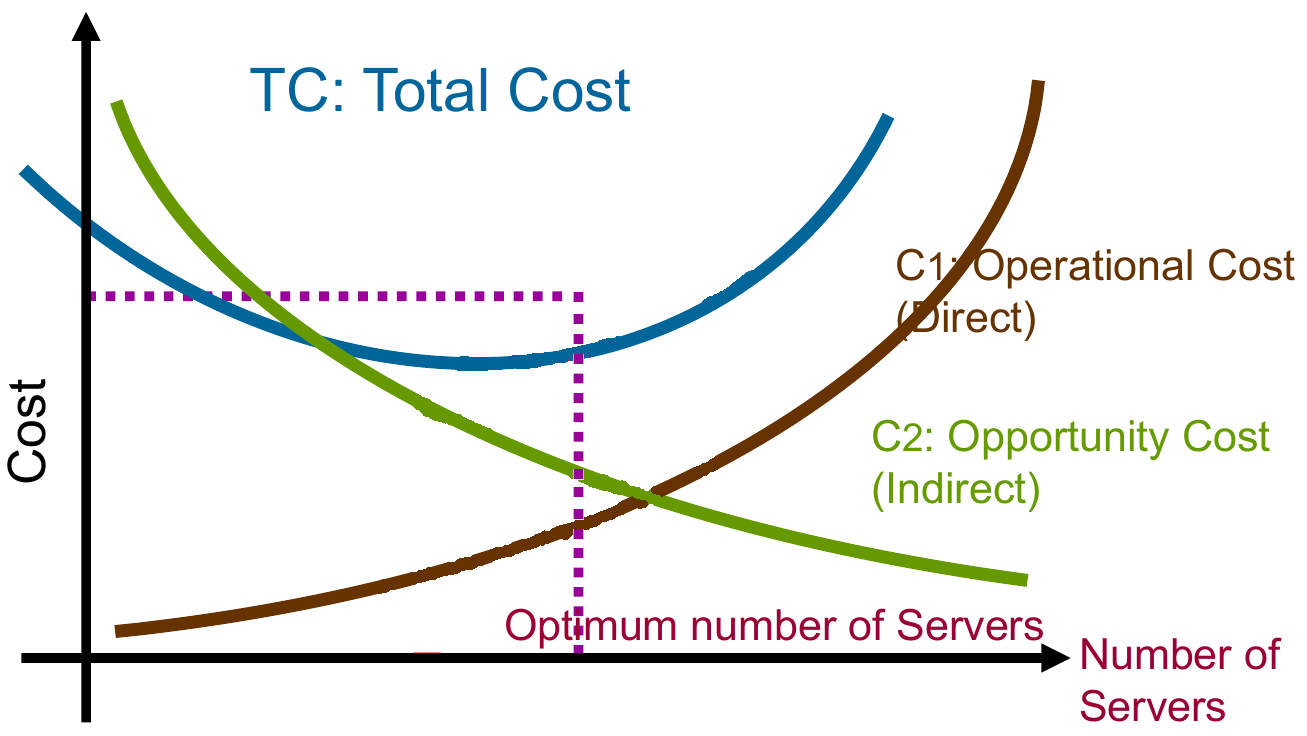
\includegraphics[
		width=14cm,
		%height=15cm
	]{images/Tema 2/Queuing motivation.png}
	\caption{
		\label{fig:unit2_qtheory}
		Queueing theory
	}
\end{figure}

\subsection{Queueing systems}

\subsubsection{Basis}

A queueing system manages traffic for a population requesting it.

Traffic is the amount of service time that has been provided to users along a period of time, so it is measured in Erlangs (E), where the unit (1 E) represents a single service being served along time, this is, the service time corresponds to time along it is being served.

A queueing system is parametrized through characteristics that are related to traffic management, such as number of users, load pattern, service characteristics and number of servers. We must then manage some performance criteria, like waiting time, blocking probability and costs.

\subsubsection{Parameters}

The parameters characterizing a queueing system are the following (some of them are redundant since they represent the same information but in another way):

\begin{itemize}
	\item Arriving rate ($u$): Amount of incoming traffic. Random variable.
	\item {
		Mean arriving rate ($\lambda$): Mean value of amount of incoming traffic:

		$ E\{u\} = \lambda $
	}
	\item {
		Time between arrivals (r): Amount of time that passes between requested services. Random variable. Its average value can be estimated from mean arriving rate:

		$ r = \frac{1}{u} \rightarrow E\{r\} = \frac{1}{\lambda} $
	}
	\item Blocking probability ($P_B$): Probability of system being stopped.
	\item {
		Effective arrival rate ($\lambda_a$): Amount of incoming traffic if we discard the traffic that can't enter the queue due to blocking phenomenom.

		$ \lambda_a = \lambda \cdot ( 1 - P_B ) $
	}
	\item {
		Queue discipline (z): It is the way in which traffic is enqueued. Most common disciplines are:

		\begin{itemize}
			\item {
				First In First Out (FIFO) / First Come First Served (FCFS): A common queue, the first element that arrived is the first element that leaves the queue.

				\begin{figure}[H]
					\centering
					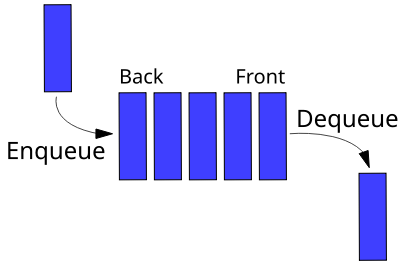
\includegraphics[
						width=7cm,
						%height=15cm
					]{images/Tema 2/Data_Queue.png}
					\caption{
						\label{fig:unit2_fifo}
						FIFO
					}
				\end{figure}
			}
			\item {
				Last in First Out (LIFO) / Last Come First Served (LCFS): A common stack, the last element that arrived is the first element that leaves the queue.

				\begin{figure}[H]
					\centering
					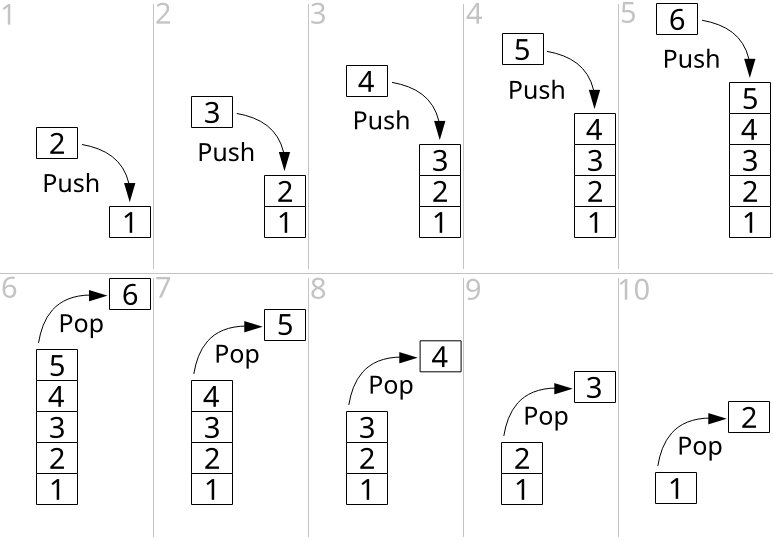
\includegraphics[
						width=8cm,
						%height=15cm
					]{images/Tema 2/Lifo_stack.png}
					\caption{
						\label{fig:unit2_lifo}
						LIFO
					}
				\end{figure}
			}
			\item Service In Random Order (SIRO): The next element leaving the system is randomly selected.
		\end{itemize}
	}
	\item Service rate ($\mu$): Rate services are completed at.
	\item {
		Service time ($s$). The amount of time a service takes to be completed. Random variable. Its average value can be estimated from service rate:

		$ E\{s\} = \frac{1}{\mu} $
	}
	\item Number of servers ($c$): Number of serving machines to attend incoming traffic.
\end{itemize}

\begin{figure}[H]
	\centering
	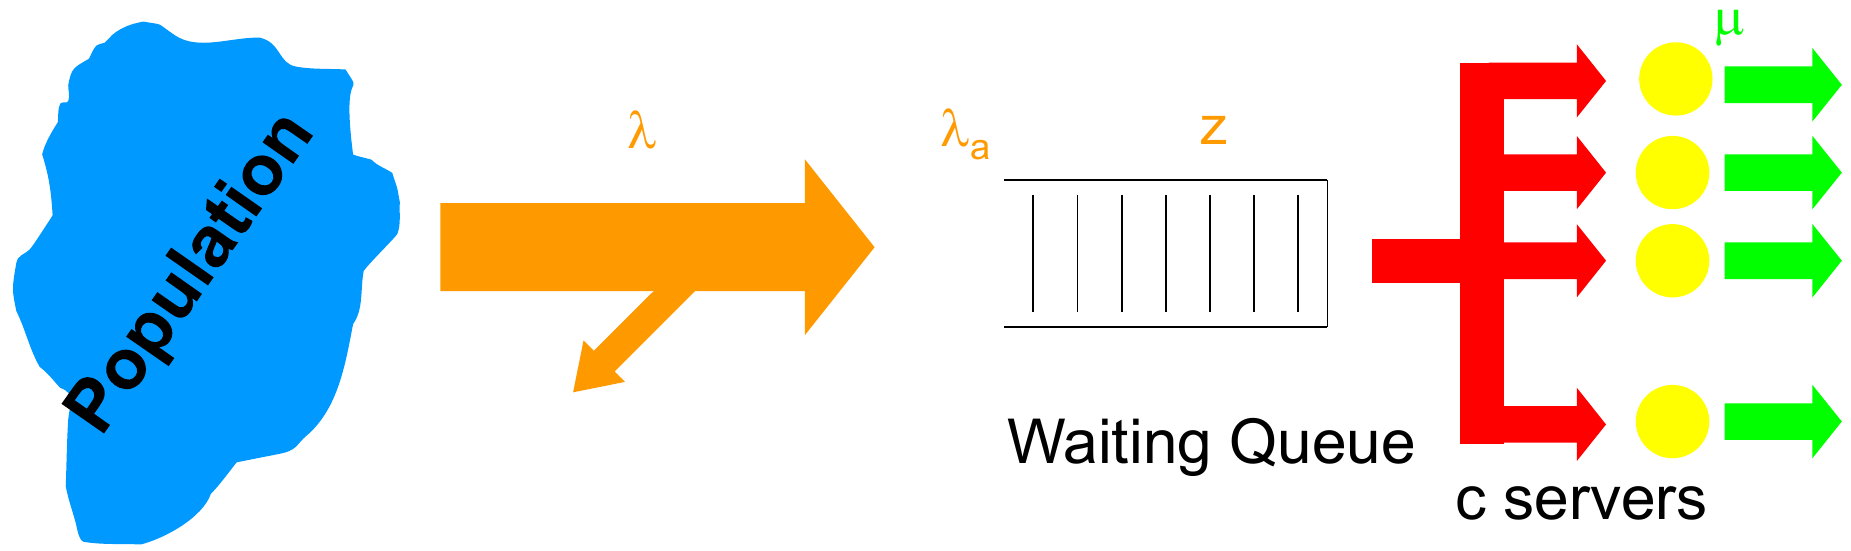
\includegraphics[
		width=12cm,
		%height=15cm
	]{images/Tema 2/Queuing system.png}
	\caption{
		\label{fig:unit2_qsystem}
		Queuing system
	}
\end{figure}

\subsubsection{Derived magnitudes}

Apart from paramaters, some aditional magnitudes derived from parameters will be useful when analyzing performance and developing solutions:

\begin{itemize}
	\item {
		Offered traffic ($A_o$): It is the amount of traffic that is said to be dispatched.

		$ A_o = \frac {E\{s\}} {E\{r\}} = \frac {\lambda} {\mu}$
	}
	\item {
		Carried traffic ($A_c$): It is the amount of traffic that is finally dispatched due to blocking phenomenom.

		$ A_c = A_o \cdot ( 1 - P_B ) = \frac {\lambda_a} {\mu} = \frac {\lambda_a} {\mu} $
	}
	\item {
		Server utilization ($\rho$):

		$ \rho = \frac {A_c} {c} = \frac {\lambda_a} {\mu \cdot c} $
	}
	\item Number of users in the servers at instant $t$ ($N_s(t)$).
	\item Number of users in the queue at instant $t$ ($N_q(t)$).
	\item {
		Number of users in the system at instant $t$ ($N(t)$):

		$ N(t) = N_s(t) + N_q(t) $
	}
	\item Number of users in the servers in continuous operation (steady state stationary regime) ($N_s$).
	\item Number of users in the queue in continuous operation (steady state stationary regime) ($N_q$).
	\item {
		Number of users in the system in continuous operation (steady state stationary regime) ($N$):

		$ N = N_s + N_q $
	}
	\item {
		Average number of users in the servers ($L_s$):

		$ L_s = E\{N_s\} $
	}
	\item {
		Average number of users in the queue ($L_q$):

		$ L_q = E\{N_q\} $
	}
	\item {
		Average number of users in the system ($L$):

		$ L = E\{N\} = L_s + L_q $
	}
	\item {
		Long-term average effective arrival rate ($\gamma$): Although this magnitude is used to demostrate Little's Law, in most of problems can be assumed to be the same as effective arrival rate $\lambda_a$.

		$ \gamma = \left. \lambda_a} \right|_{\textrm{long-term}} $
	}
	\item {
		Mean time in the servers ($W_s$):

		$ W_s = E\{s\} = \frac{1}{\mu} = \frac{L_s}{\gamma} $
	}
	\item {
		Mean time in the queue ($W_q$):

		$ W_q = \frac {L_q} {\gamma} $
	}
	\item {
		Mean time in the system ($W$):

		$ W = W_s + W_q = \frac {L} {\gamma} $
	}
\end{itemize}

\subsubsection{Little's Law}

Little's Law relates the number of users in the system with traffic. Little proved that the long-term average number of users in the servers is equal to carried traffic:

$$
	\begin{Bmatrix}
		L_s = \gamma \cdot W_s \\
		L_q = \gamma \cdot W_q
	\end{Bmatrix}
	\rightarrow
$$

$$
	\rightarrow
	L = L_s + L_q = \gamma \cdot W_s + \gamma \cdot W_q = \gamma \cdot W
	\rightarrow
$$

$$
	\rightarrow
	\left. A_c \right|_{\textrm{long-term}} = \left. \frac {\lambda_a} {\mu} \right|_{\textrm{long-term}} = \gamma \cdot W_s = L_s
$$

\subsubsection{Kendall-Lee notation}

Having a common set of defining parameters, queueing models can be refered through a common notation. We use Kendall-Lee notation:

$$
	A / B / c / K / m / z
$$

Parameters of this notation are:

\begin{itemize}
	\item {
		Arrival process ($A$): It specifies the distribution of arrival rate ($r$). Some common distributions are:
		\begin{itemize}
			\item $M$: Independent and identically distributed random variable with Poisson distribution (time between arrivals follows an exponential distribution).
			\item $D$: Independent and identically distributed random variable with determinist distribution.
			\item $GI$: Independent and identically distributed random variable with general distribution.
		\end{itemize}
	}
	\item {
		Service time distribution ($B$): It specifies the distribution of service time ($s$). Some common distributions are:
		\begin{itemize}
			\item $M$: Independent and identically distributed random variable with exponential distribution.
			\item $D$: Independent and identically distributed random variable with determinist distribution.
			\item $GI$: Independent and identically distributed random variable with general distribution.
		\end{itemize}
	}
	\item Number of servers ($c$): The number of service channels (or servers).
	\item Capacity of queue ($K$): Maximum number of customers allowed in the queue. When the number is at this maximum, further arrivals are turned away. If this number is omitted, the capacity is assumed to be infinite.
	\item Population size ($m$): The size of the population from which the customers come. If this number is omitted, the population is assumed to be unlimited, or infinite.
	\item Queue discipline ($z$): As seen in \textit{Parameters} section, it is the way in which traffic is enqueued and can be of three types, FIFO, LIFO and SIRO. When omitted, discipline is assumed to be FIFO.
\end{itemize}

\subsection{Common distributions at queueing systems}

\subsubsection{Exponential distribution}

The service time usually follows an exponential distribution, this is, we can estimate the probability that a user spends a time $t$ to be served with the density function $p_s(t)$. This also means that $p_s(t) \cdot 100\%$ of user will take a time $t$ to be served. We define the density function:

$$
	s \sim exp(\mu) \leftrightarrow P(s = t) = p_s(t) =
	\begin{Bmatrix}
		\mu \cdot e^{- \mu \cdot t}, 0 < t \\
		0, t \leq 0
	\end{Bmatrix}
	\rightarrow
	E\{s\} = \frac{1}{\mu}
$$

\begin{figure}[H]
	\centering
	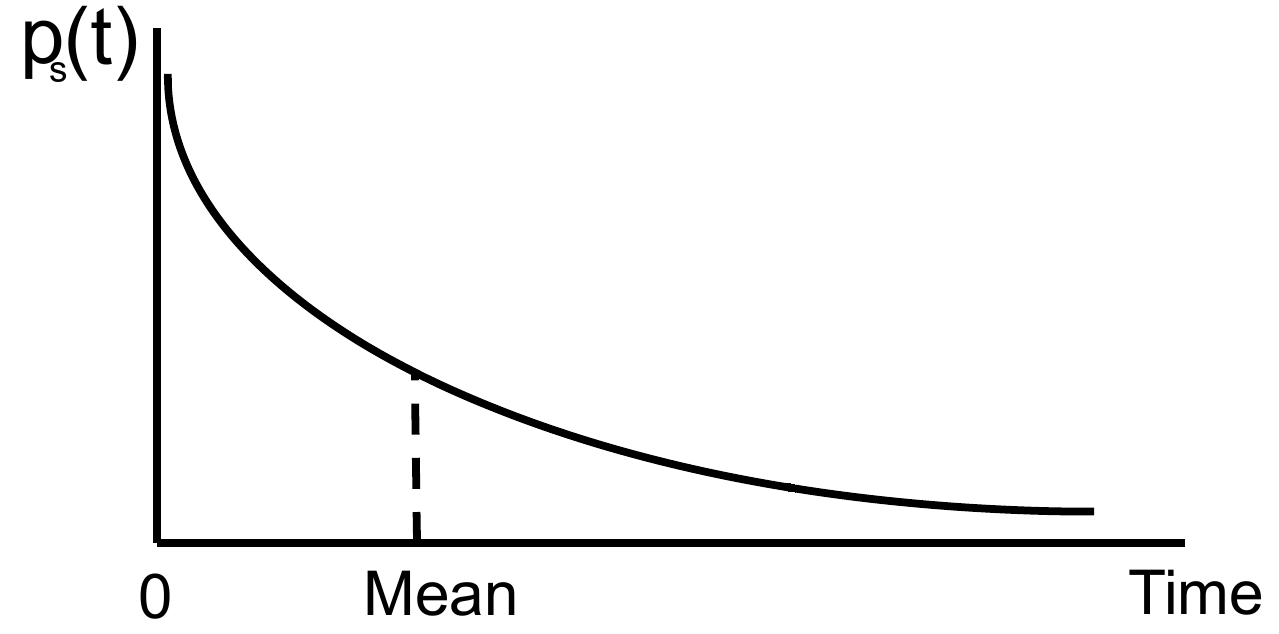
\includegraphics[
		width=10cm,
		%height=15cm
	]{images/Tema 2/Exponential distribution.png}
	\caption{
		\label{fig:unit2_exp}
		Exponential distribution
	}
\end{figure}

Distribution function can also be computed:

$$
	P(s \leq T) =
	P_s(T) =
	\int_{-\infty}^{T} p_s(t) dt =
	\int_{0}^{T} \mu \cdot e^{- \mu \cdot t} dt =
	1 - e^{- \mu \cdot t}
$$

\begin{figure}[H]
	\centering
	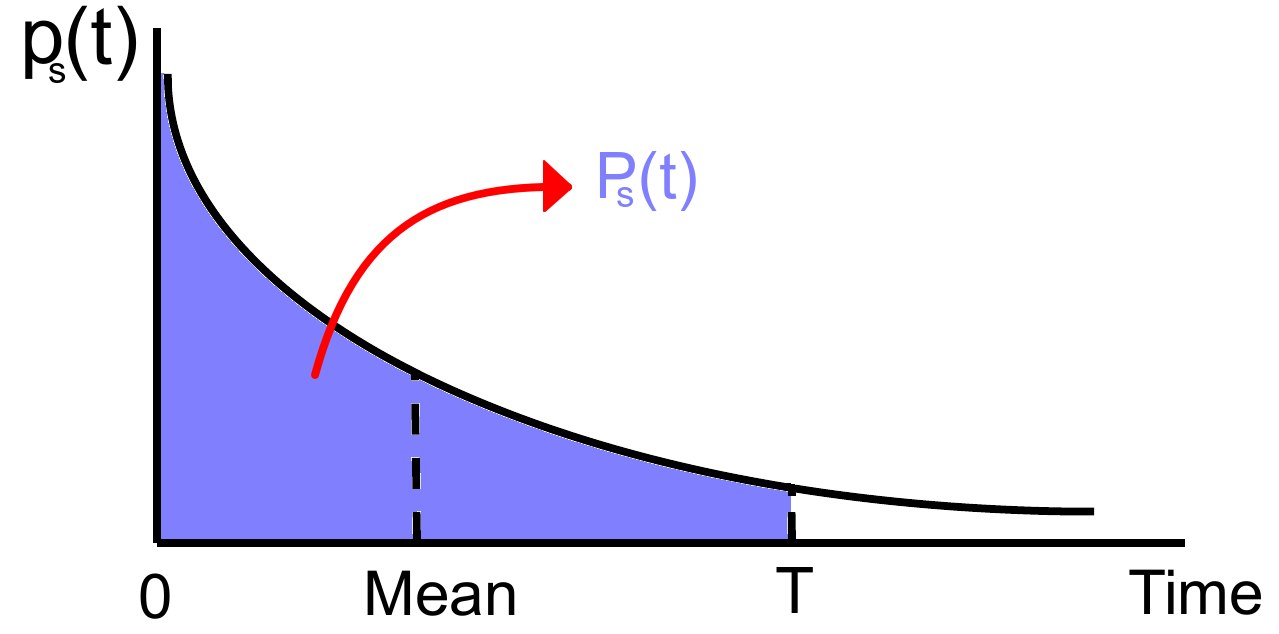
\includegraphics[
		width=10cm,
		%height=15cm
	]{images/Tema 2/Exponential distribution with area.png}
	\caption{
		\label{fig:unit2_exp_area}
		Exponential distribution area
	}
\end{figure}

\subsubsection{Poisson distribution}

Arrival rate is usually modeled by a Poisson distribution, this is, we can estimate the probability of $k$ arrivals within a unit of time with the density function. This is because we consider that time between arrivals follows an exponential distribution:

$$
	r \sim exp(\lambda) \rightarrow
	u \sim Poi(\lambda) \leftrightarrow
	P(u = k) = p_u(k) =
	\frac {\lambda^k \cdot e^{-k}} {k!} \rightarrow
	E\{u\} = \lambda
$$

\begin{figure}[H]
	\centering
	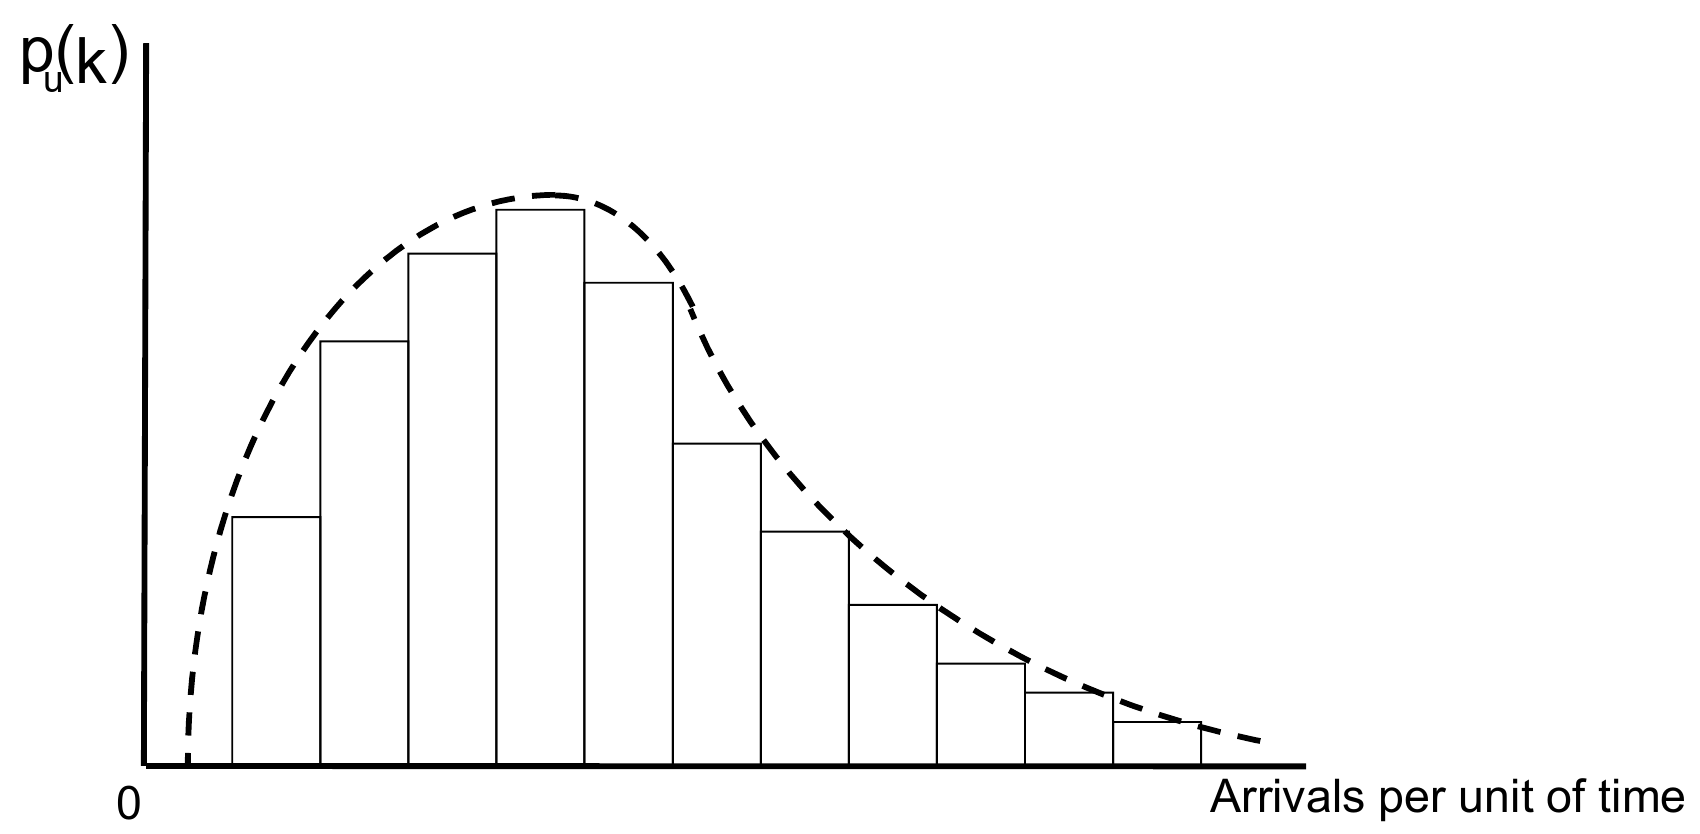
\includegraphics[
		width=10cm,
		%height=15cm
	]{images/Tema 2/Poisson distribution.png}
	\caption{
		\label{fig:unit2_poi}
		Poisson distribution
	}
\end{figure}

\subsection{Basic queueing models}

\subsubsection{$M/M/1$ model}

\paragraph{Characteristics}

The characteristics of this model are:

\begin{itemize}
	\item {
		Time between arrivals follows exponential distribution, then, arrivals rate follows Poisson distribution:

		$
			A = M \rightarrow r \sim exp(\lambda) \rightarrow u \sim Poi(\lambda)
		$
	}
	\item {
		Service time follows exponential distribution:

		$
			B = M \rightarrow s \sim exp(\mu)
		$
	}
	\item {
		One server:

		$
			c = 1
		$
	}
	\item {
		Infinite queue capacity:

		$
			K = \infty
		$
	}
	\item {
		Infinite population:

		$
			m = \infty
		$
	}
	\item {
		FIFO queue.

		$
			z = FIFO
		$
	}
	\item A certain blocking probability ($P_B$).
\end{itemize}

\begin{figure}[H]
	\centering
	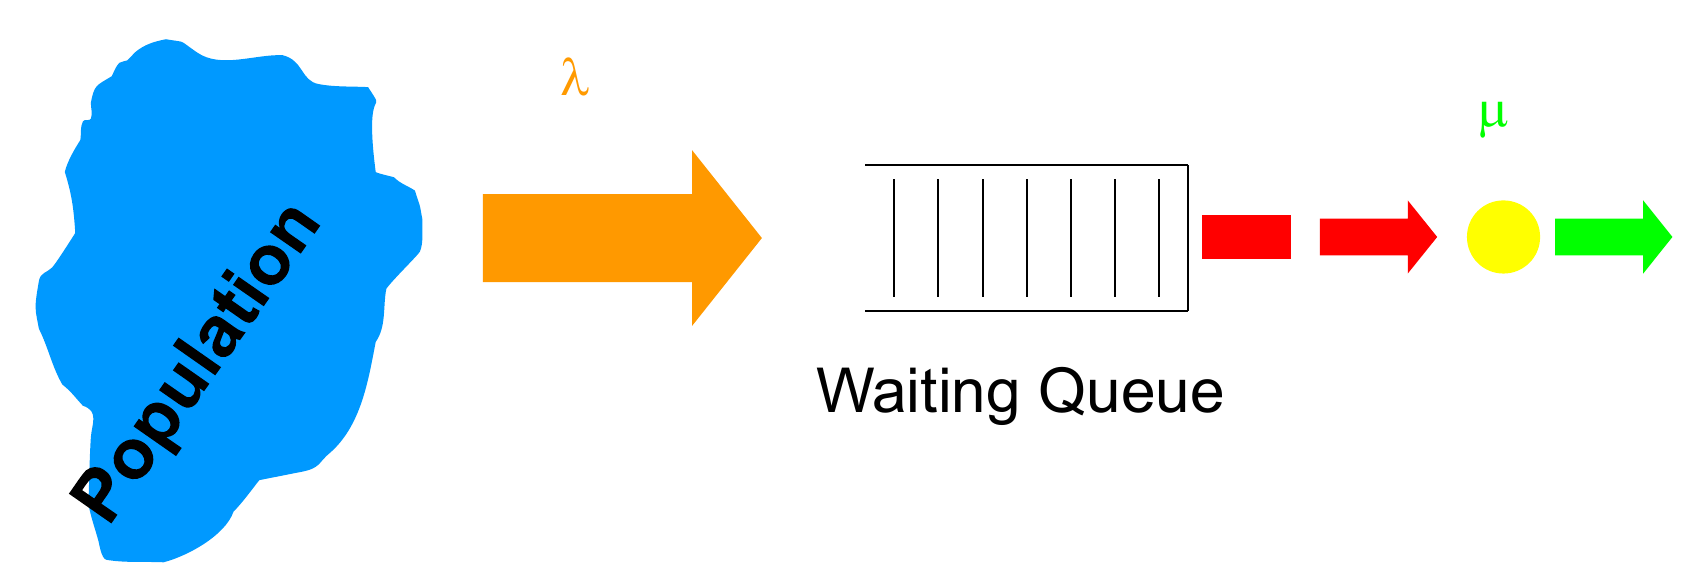
\includegraphics[
		width=12cm,
		%height=15cm
	]{images/Tema 2/M⁄M⁄1 model.png}
	\caption{
		\label{fig:unit2_MM1}
		M/M/1 model
	}
\end{figure}

\begin{figure}[H]
	\centering
	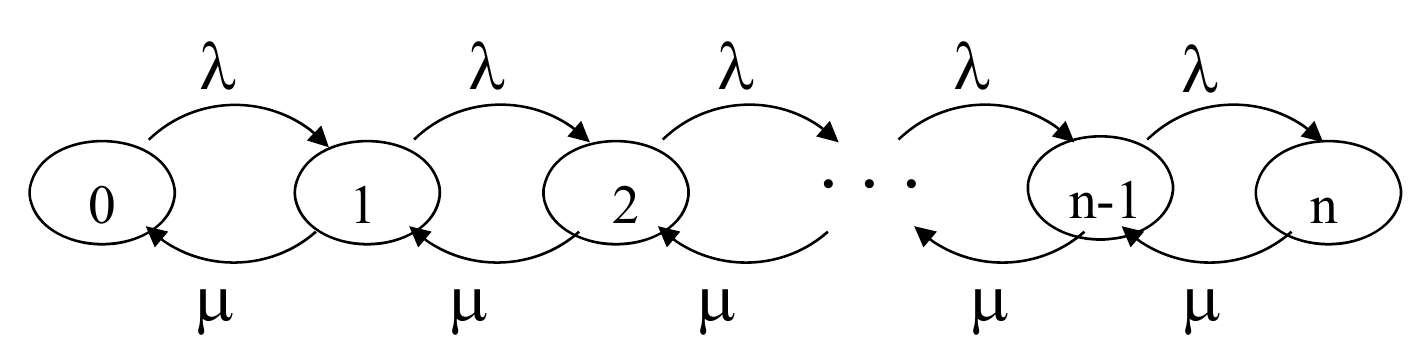
\includegraphics[
		width=12cm,
		%height=15cm
	]{images/Tema 2/MM1 model queue.png}
	\caption{
		\label{fig:unit2_MM1_queue}
		M/M/1 model queue
	}
\end{figure}

\paragraph{Properties}

The rest of properties can be derived:

\begin{itemize}
	\item {
		Server utilization (it must be less than one in order to have an stable system):

		$
			\rho =
			\frac {\lambda_a} {\mu \cdot c} \overset {\textrm{long-term}} {=}
			\frac {\gamma} {\mu \cdot c} \overset {c=1} {=}
			\frac {\gamma} {\mu} =
			\gamma \cdot W_s =
			L_s =
			\left. A_c \right|_{\textrm{long-term}} < 1
		$
	}
	\item {
		Summation $S$:

		$
			S =
			\sum_{n=0}^{\infty} \left( \frac {\lambda} {\mu} \right)^n =
			\sum_{n=0}^{\infty} A_o^n =
			\sum_{n=0}^{\infty} \left( \frac {A_c} {1 - P_B} \right)^n =
			\sum_{n=0}^{\infty} \left( \frac {c \cdot \rho} {1 - P_B} \right)^n \overset {c=1, P_B=0} {=}
			\sum_{n=0}^{\infty} \rho^n =
			\frac {1} {1 - \rho}
		$
	}
	\item {
		Probability of the server not being used:

		$
			P_0 = \frac {1} {S} = 1 - \rho
		$
	}
	\item {
		Probability of the server being used:

		$
			P(n \geq 1) = 1 - P_0 = \rho
		$
	}
	\item {
		Probability of the server being in any state:

		$
			P(n \geq 1) = \rho = \sum_{n=1}^{\infty} P_n \rightarrow P_n = (1 - \rho) \cdot \rho^n
		$
	}
	\item {
		Average number of users in the servers:

		$
			L_s = \gamma \cdot W_s = \frac {\gamma} {\mu} = \rho
		$
	}
	\item {
		Average number of users in the queue:

		$
			L_q = \sum_{i=1}^{\infty} \left[ (i-1) \cdot P_i \right] =
			\sum_{i=1}^{\infty} \left[ (i-1) \cdot (1-\rho) \cdot \rho^i \right] =
			\frac {\rho^2} {1-\rho}
		$
	}
	\item {
		Average number of users in the system:

		$
			L = \sum_{i=1}^{\infty} \left[ i \cdot P_i \right] =
			\sum_{i=1}^{\infty} \left[ i \cdot (1-\rho) \cdot \rho^i \right] =
			\frac {\rho} {1-\rho}
		$
	}
	\item {
		Mean time in servers:

		$
			W_s = \frac {1} {\mu}
		$
	}
	\item {
		Mean time in the queue:

		$
			W_q = \frac {L_q} {\gamma} = \frac {\frac{\rho^2}{1-\rho}} {\frac{\rho}{W_s}} =
			W_s \cdot \frac {\rho} {1-\rho} =
			\frac {\rho} {\mu \cdot (1-\rho)} \overset {\rho=1} {=} \infty
		$
	}
	\item {
		Mean time in the system:

		$
			W =
			W_s + W_q =
			W_s + W_s \cdot \frac {\rho} {1-\rho} =
			\frac {W_s} {1-\rho} =
			\frac {1} {\mu \cdot (1-\rho)} \overset {\rho=1} {=} \infty
		$
	}
\end{itemize}

\subsubsection{$M/M/c$ model}

\paragraph{Characteristics}

The characteristics of this model are:

\begin{itemize}
	\item {
		Time between arrivals follows exponential distribution, then, arrivals rate follows Poisson distribution:

		$
			A = M \rightarrow r \sim exp(\lambda) \rightarrow u \sim Poi(\lambda)
		$
	}
	\item {
		Service time follows exponential distribution:

		$
			B = M \rightarrow s \sim exp(\mu)
		$
	}
	\item {
		$c$ servers:

		$
			c = c
		$
	}
	\item {
		Infinite queue capacity:

		$
			K = \infty
		$
	}
	\item {
		Infinite population:

		$
			m = \infty
		$
	}
	\item {
		FIFO queue.

		$
			z = FIFO
		$
	}
	\item A certain blocking probability ($P_B$).
\end{itemize}

\begin{figure}[H]
	\centering
	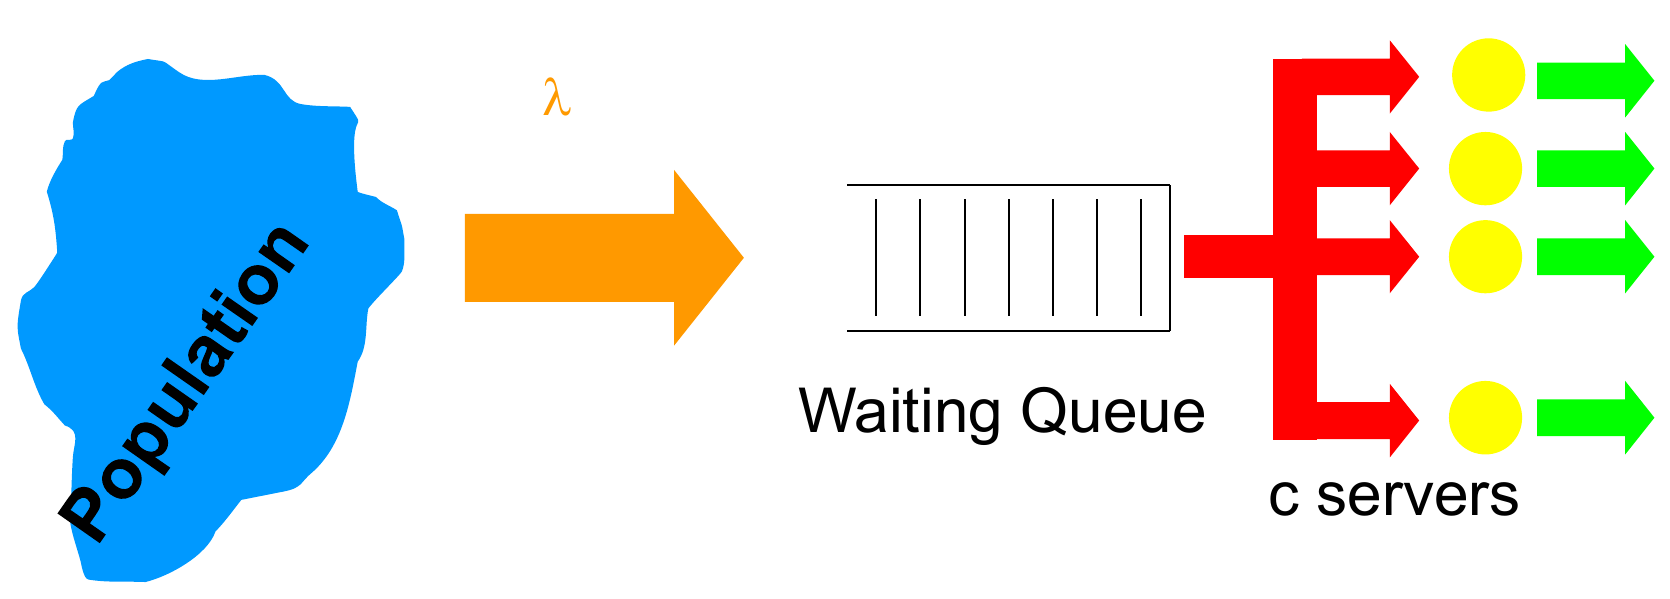
\includegraphics[
		width=12cm,
		%height=15cm
	]{images/Tema 2/M⁄M⁄c model.png}
	\caption{
		\label{fig:unit2_MMc}
		M/M/c model
	}
\end{figure}

\begin{figure}[H]
	\centering
	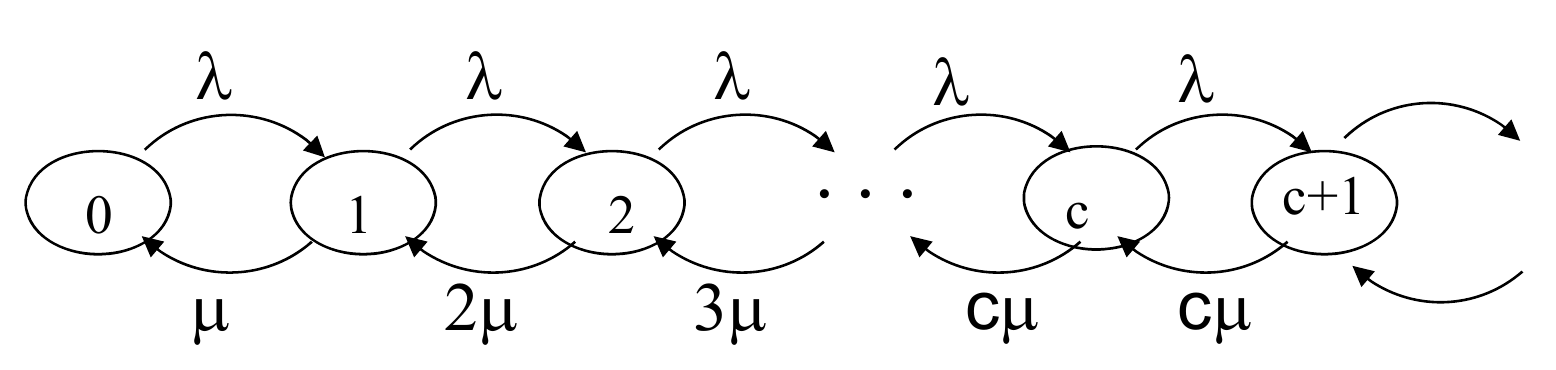
\includegraphics[
		width=12cm,
		%height=15cm
	]{images/Tema 2/MMc model queue.png}
	\caption{
		\label{fig:unit2_MMc_queue}
		M/M/c model queue
	}
\end{figure}

\paragraph{Erlang C}

As can be infered, estimating waiting time distribution in this model is more complex. The probability of a customer having to wait on the queue due to having all servers occupied can be computed iteratively with Erlang C function, which depends on the incoming offered traffic $A_o$ and the number of servers $c$:

$$
	C(A_o, c) = \frac {A_{o}^c} {c! \cdot (1-\rho)} P_0 =  \frac {A_{o}^c} { c! \cdot (1-\rho) \cdot \left( \sum_{n=0}^{c-1} \left( \frac {A_{o}^n} {n!} \right) + \frac {A_{o}^c} {c! \cdot (1-\rho)} \right) }
$$

\begin{figure}[H]
	\centering
	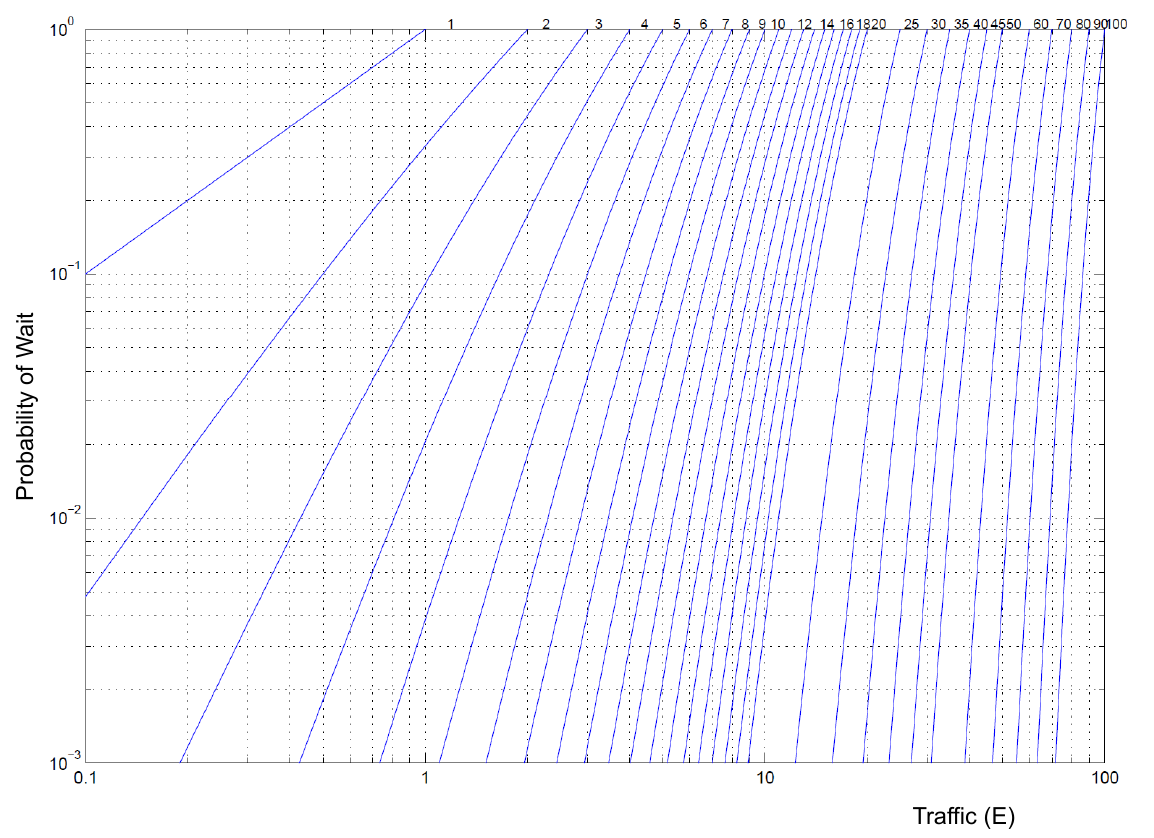
\includegraphics[
		width=14cm,
		%height=15cm
	]{images/Tema 2/Erlang C.png}
	\caption{
		\label{fig:unit2_erlangC}
		Erlang C for M/M/c model
	}
\end{figure}

\paragraph{Properties}

The rest of properties can be derived:

\begin{itemize}
	\item {
		Server utilization (it must be less than one in order to have an stable system):

		$
			\rho =
			\frac {\lambda_a} {\mu \cdot c} \overset {\textrm{long-term}} {=}
			\frac {\gamma} {\mu \cdot c} =
			\frac {\gamma \cdot W_s} {c} =
			\frac {L_s} {c} =
			\frac {\left. A_c \right|_{\textrm{long-term}}} {c}
			< 1
		$
	}
	\item {
		Summation $S$:

		$
			S =
			\sum_{n=0}^{c-1} \left( \frac {A_{o}^n} {n!} \right) + \frac {A_{o}^c} {c! \cdot (1-\rho)}
		$
	}
	\item {
		Probability of the server not being used:

		$
			P_0 = \frac {1} {S} = \frac {1} {\sum_{n=0}^{c-1} \left( \frac {A_{o}^n} {n!} \right) + \frac {A_{o}^c} {c! \cdot (1-\rho)}}
		$
	}
	\item {
		Probability of the server being used:

		$
			P(n \geq 1) = 1 - P_0 = 1 - \frac {1} {S}
		$
	}
	\item {
		Probability of the server being in any state:

		$
			P(n \geq 1) = 1 - \frac {1} {S} = \sum_{n=1}^{\infty} P_n \rightarrow
			P_n = \frac {1} {S} \cdot \left( 1 - \frac {1} {S} \right)^n
		$
	}
	\item {
		Probability of having to wait in the queue:

		$
			P_{wait} = C(A_o, c) = \frac {A_{o}^c} {c! \cdot (1-\rho)} P_0 =  \frac {A_{o}^c} { c! \cdot (1-\rho) \cdot \left( \sum_{n=0}^{c-1} \left( \frac {A_{o}^n} {n!} \right) + \frac {A_{o}^c} {c! \cdot (1-\rho)} \right) }
		$
	}
	\item {
		Average number of users in the servers:

		$
			L_s = \gamma \cdot W_s = \frac {\gamma} {\mu} = c \cdot \rho
		$
	}
	\item {
		Average number of users in the queue:

		$
			L_q = \frac {\rho} {1-\rho} \cdot C(A_o, c)
		$
	}
	\item {
		Average number of users in the system:

		$
			L = c \cdot \rho + \frac {\rho} {1-\rho} \cdot C(A_o, c)
		$
	}
	\item {
		Mean time in servers:

		$
			W_s = \frac {1} {\mu}
		$
	}
	\item {
		Mean time in the queue:

		$
			W_q =
			\frac {W_s} {c \cdot (1-\rho)} \cdot C(A_o, c) =
			\frac {1} {\mu \cdot c \cdot (1-\rho)} \cdot C(A_o, c)
		$
	}
	\item {
		Mean time in the system:

		$
			W =
			W_s + W_q =
			W_s + \frac {W_s} {c \cdot (1-\rho)} \cdot C(A_o, c) =
			\frac {1} {\mu} + \frac {1} {\mu \cdot c \cdot (1-\rho)} \cdot C(A_o, c)
			\overset {\rho=1} {=} \infty
		$
	}
	\item {
		Distribution of mean time in the queue:

		$
			P(W_q < t) = 1 - C(A_o, c) \cdot e^{- c \cdot \mu \cdot (1-\rho) \cdot t}
		$
	}
\end{itemize}

\subsubsection{$M/M/c/c$ model}

\paragraph{Characteristics}

The characteristics of this model are:

\begin{itemize}
	\item {
		Time between arrivals follows exponential distribution, then, arrivals rate follows Poisson distribution:

		$
			A = M \rightarrow r \sim exp(\lambda) \rightarrow u \sim Poi(\lambda)
		$
	}
	\item {
		Service time follows exponential distribution:

		$
			B = M \rightarrow s \sim exp(\mu)
		$
	}
	\item {
		$c$ servers:

		$
			c = c
		$
	}
	\item {
		Queue capacity is limited to number of servers:

		$
			K = c
		$
	}
	\item {
		Infinite population:

		$
			m = \infty
		$
	}
	\item {
		FIFO queue.

		$
			z = FIFO
		$
	}
	\item A certain blocking probability ($P_B$).
\end{itemize}

\begin{figure}[H]
	\centering
	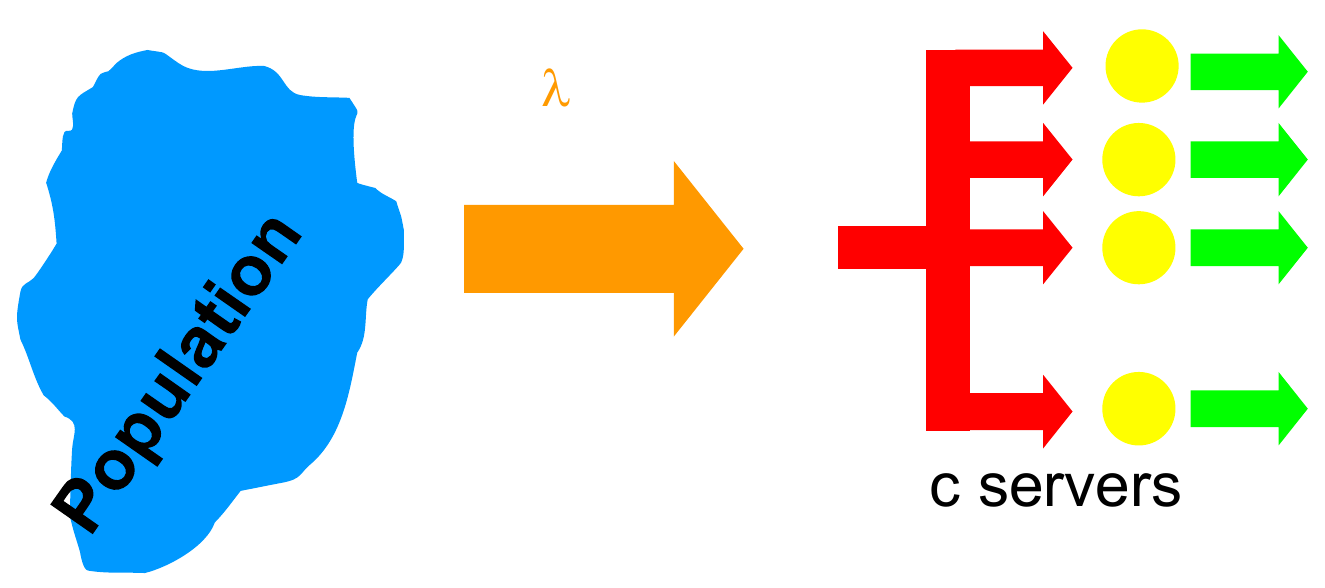
\includegraphics[
		width=12cm,
		%height=15cm
	]{images/Tema 2/M⁄M⁄c⁄c model.png}
	\caption{
		\label{fig:unit2_MMcc}
		M/M/c/c model
	}
\end{figure}

\begin{figure}[H]
	\centering
	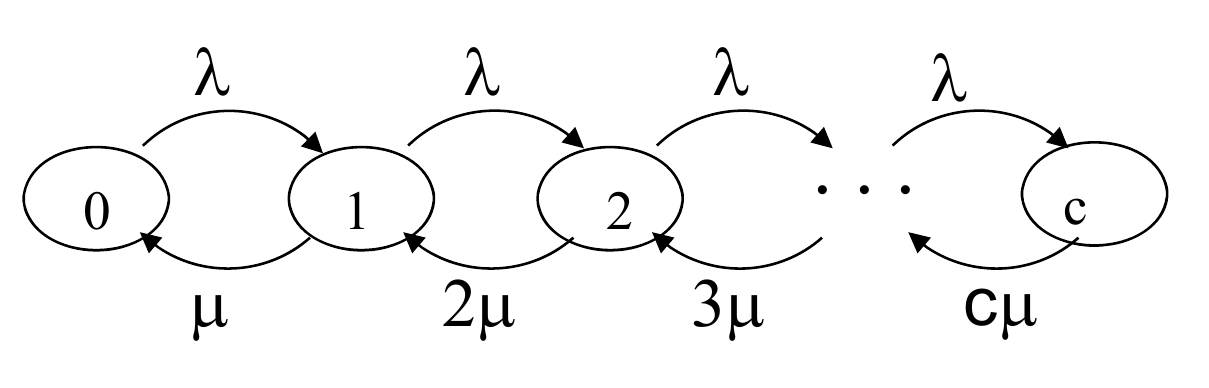
\includegraphics[
		width=12cm,
		%height=15cm
	]{images/Tema 2/MMcc model queue.png}
	\caption{
		\label{fig:unit2_MMcc_queue}
		M/M/c/c model queue
	}
\end{figure}

\paragraph{Erlang B}

The fact that the queue has the same size as the number of servers equals to not having queue but a fixed number of $c$ servers. As can be infered, apart from external blocking sources, this system itself will cause blocking when there are more calls than available servers. Blocking probability can be computed iteratively with Erlang B function, which depends on the incoming offered traffic $A_o$ and the number of servers $c$:

$$
	B(A_o, c) = P_0 \cdot \frac {A_{o}^c} {c!}= \frac {A_{o}^c} { c! \cdot \left( \sum_{n=0}^{c} \left( \frac {A_{o}^n} {n!} \right) \right) }
$$

\begin{figure}[H]
	\centering
	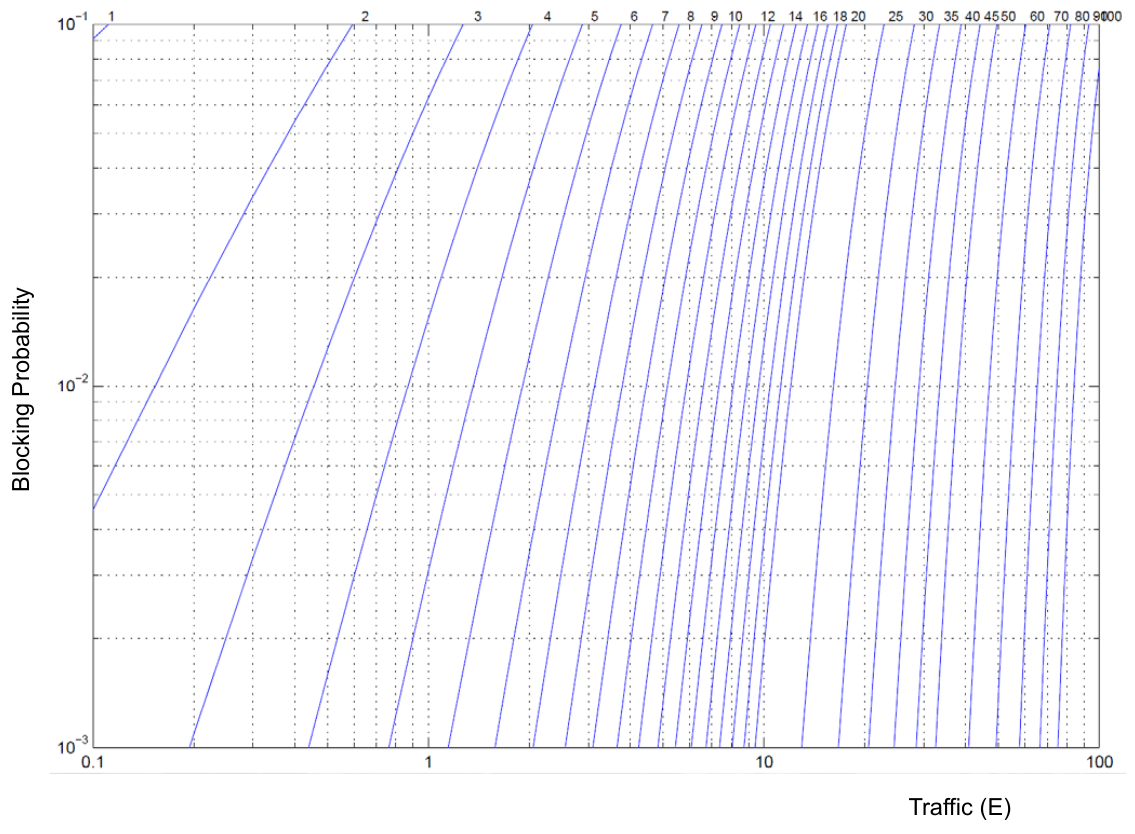
\includegraphics[
		width=14cm,
		%height=15cm
	]{images/Tema 2/Erlang B.png}
	\caption{
		\label{fig:unit2_erlangB}
		Erlang B for M/M/c/c model
	}
\end{figure}

\paragraph{Properties}

The rest of properties can be derived:

\begin{itemize}
	\item {
		Server utilization (it must be less than one in order to have an stable system):

		$
			\rho =
			\frac {\lambda_a} {\mu \cdot c} \overset {\textrm{long-term}} {=}
			\frac {\gamma} {\mu \cdot c} =
			\frac {\gamma \cdot W_s} {c} =
			\frac {L_s} {c} =
			\frac {\left. A_c \right|_{\textrm{long-term}}} {c}
			< 1
		$
	}
	\item {
		Summation $S$:

		$
			S = \sum_{n=0}^{c} \left( \frac {A_{o}^n} {n!} \right)
		$
	}
	\item {
		Probability of the server not being used:

		$
			P_0 = \frac {1} {S} = \frac {1} {\sum_{n=0}^{c} \left( \frac {A_{o}^n} {n!} \right)}
		$
	}
	\item {
		Probability of the server being used:

		$
			P(n \geq 1) = 1 - P_0 = 1 - \frac {1} {S}
		$
	}
	\item {
		Probability of the server being in any state:

		$
			P(n \geq 1) = 1 - \frac {1} {S} = \sum_{n=1}^{\infty} P_n \rightarrow
			P_n = \frac {1} {S} \cdot \left( 1 - \frac {1} {S} \right)^n =
			P_0 \cdot \frac {A_{o}^n} {c!} = \frac {\frac{A_{o}^n}{c!}} {\sum_{k=0}^c \left( \frac {A_{o}^k} {k!} \right)}
		$
	}
	\item {
		Probability of the server being in any state:

		$
			P(n \geq 1) = 1 - \frac {1} {S} = \sum_{n=1}^{\infty} P_n \rightarrow
			P_n = \frac {1} {S} \cdot \left( 1 - \frac {1} {S} \right)^n
		$
	}
	\item {
		Probability of having to wait in the queue:

		$
			P_{wait} = 0
		$
	}
	\item {
		Blocking probability:

		$
			P_{\textrm{blocking}} = B(A_o, c) = P_0 \cdot \frac {A_{o}^c} {c!} = \frac {\frac{A_{o}^c}{c!}} {\sum_{n=0}^c \left( \frac {A_{o}^n} {n!} \right)} = \frac {A_{o}^c} { c! \cdot \left( \sum_{n=0}^{c} \left( \frac {A_{o}^n} {n!} \right) \right) }
		$
	}
	\item {
		Carried traffic:

		$
			A_c = A_o \cdot \left( 1 - B(A_o, c) \right)
		$
	}
	\item {
		Average number of users in the servers:

		$
			L_s = \gamma \cdot W_s = \frac {\gamma} {\mu} = c \cdot \rho
		$
	}
	\item {
		Average number of users in the queue:

		$
			L_q = 0
		$
	}
	\item {
		Average number of users in the system:

		$
			L = L_s = c \cdot \rho
		$
	}
	\item {
		Mean time in servers:

		$
			W_s = \frac {1} {\mu}
		$
	}
	\item {
		Mean time in the queue:

		$
			W_q = 0
		$
	}
	\item {
		Mean time in the system:

		$
			W =
			W_s + W_q =
			W_s =
			\frac {1} {\mu}
		$
	}
\end{itemize}

\subsubsection{Summary}

\begin{tabular}{|c|c|c|c|}
	\hline
	& $M/M/1$ & $M/M/c$ & $M/M/c/c$ \\
	\hline
	$A$ & \multicolumn{3}{c|}{$M$} \\
	\hline
	$B$ & \multicolumn{3}{c|}{$M$} \\
	\hline
	$c$ & $1$ & \multicolumn{2}{c|}{$c$} \\
	\hline
	$K$ & \multicolumn{2}{c|}{$\infty$} & $c$ \\
	\hline
	$m$ & \multicolumn{3}{c|}{$\infty$} \\
	\hline
	$z$ & \multicolumn{3}{c|}{$FIFO$} \\
	\hline
	$r$ & \multicolumn{3}{c|}{$\sim exp(\lambda)$} \\
	\hline
	$u$ & \multicolumn{3}{c|}{$\sim Poi(\lambda)$} \\
	\hline
	$s$ & \multicolumn{3}{c|}{$\sim exp(\mu)$} \\
	\hline
\end{tabular}

\begin{landscape}

\begin{tabular}{|c|c|c|c|}
	\hline
	& $M/M/1$ & $M/M/c$ & $M/M/c/c$ \\
	\hline
	$\rho$ & $\frac {\lambda_a} {\mu} = A_c = L_s < 1$ & \multicolumn{2}{c|}{$\frac {\lambda_a} {\mu \cdot c} = \frac {A_c} {c} = \frac {L_s} {c} < 1$} \\
	\hline
	$S$ & $\frac {1} {1 - \rho}$ & $\sum_{n=0}^{c-1} \left( \frac {A_{o}^n} {n!} \right) + \frac {A_{o}^c} {c! \cdot (1-\rho)}$ & $\sum_{n=0}^{c} \left( \frac {A_{o}^n} {n!} \right)$ \\
	\hline
	$P_0$ & $\frac {1} {S} = 1 - \rho$ & $\frac {1} {S} = \frac {1} {\sum_{n=0}^{c-1} \left( \frac {A_{o}^n} {n!} \right) + \frac {A_{o}^c} {c! \cdot (1-\rho)}}$ & $\frac {1} {S} = \frac {1} {\sum_{n=0}^{c} \left( \frac {A_{o}^n} {n!} \right)}$ \\
	\hline
	$P(n \geq 1)$ & $1 - P_0 = \rho$ & $1 - P_0$ & $1 - P_0$ \\
	\hline
	$P_n$ & $(1 - \rho) \cdot \rho^n$ & $\frac {1} {S} \cdot \left( 1 - \frac {1} {S} \right)^n$ & $\frac {\frac{A_{o}^n}{c!}} {\sum_{k=0}^c \left( \frac {A_{o}^k} {k!} \right)}$ \\
	\hline
	$L_s$ & $A_c = \frac {\lambda_a} {\mu} = \rho$ & \multicolumn{2}{c|}{$A_c = \frac {\lambda_a} {\mu} = c \cdot \rho$} \\
	\hline
	$L_q$ & $\frac {\rho^2} {1-\rho}$ & $\frac {\rho} {1-\rho} \cdot C(A_o, c)$ & $0$ \\
	\hline
	$L$ & $\frac {\rho} {1-\rho}$ & $c \cdot \rho + \frac {\rho} {1-\rho} \cdot C(A_o, c)$ & $L_s = A_c = \frac {\lambda_a} {\mu} = c \cdot \rho$ \\
	\hline
	$W_s$ & \multicolumn{3}{c|}{$\frac {1} {\mu}$} \\
	\hline
	$W_q$ & $W_s \cdot \frac {\rho} {1-\rho} = \frac {\rho} {\mu \cdot (1-\rho)}$ & $\frac {W_s} {c \cdot (1-\rho)} \cdot C(A_o, c) = \frac {1} {\mu \cdot c \cdot (1-\rho)} \cdot C(A_o, c)$ & $0$ \\
	\hline
	$W$ & $\frac {W_s} {1-\rho} = \frac {1} {\mu \cdot (1-\rho)}$ & $W_s + \frac {W_s} {c \cdot (1-\rho)} \cdot C(A_o, c) = \frac {1} {\mu} + \frac {1} {c \cdot \mu \cdot (1-\rho)} \cdot C(A_o, c)$ & $W_s = \frac {1} {\mu}$ \\
	\hline
	$P_{wait}$ & $A_o = \frac {\lambda} {\mu}$ & $C(A_o, c)$ & $0$ \\
	\hline
	$P_{blocking}$ & \multicolumn{2}{c|}{$0$} & $B(A_o, c)$ \\
	\hline
	$P(W_q < t)$ & $1 - A_o \cdot e^{- \mu \cdot (1-A_o) \cdot t}$ & $1 - C(A_o, c) \cdot e^{- c \cdot \mu \cdot (1-\rho) \cdot t}$ & \\
	\hline
	$P(W_q > t)$ & $A_o \cdot e^{- \mu \cdot (1-A_o) \cdot t}$ & $C(A_o, c) \cdot e^{- c \cdot \mu \cdot (1-\rho) \cdot t}$ & \\
	\hline
\end{tabular}

\end{landscape}

\section{Telephony network architecture}

\subsection{Hierarchical networks}

\subsubsection{Introduction}

The main reason for the usage of hierarchical networks is the reduction of the number of connections among subscribers:

\begin{itemize}
	\item If we have $N$ telephones, we need $C = \frac {N \cdot (N - 1)} {2}$ connections for interconnecting each other.
	\item If we include a local exchange for a certain area, the number of connections is reduced to $C = N$.
\end{itemize}
Each of these connections is denoted \textit{subscriber loop} or \textit{subscriber line}. The exchange that only connects subscribers from the same area is denoted \textit{local exchange} or \textit{toll center}.

\subsubsection{Hierarchy}

If toll centers were not interconnected, only local calls could be carried out. Since we need to interconnect the toll centers with each other and they are too much (thousand in Spain), a new exchange is needed, denoted as primary center. Some primary centers has also their own subscribers. The link between toll and primary centers is denoted as primary section or trunk. The primary area is defined by the primary center and everything under it (local centers and subscribers).

Again, the number of primary centers is too high and thus, a higher level exchange is defined, denoted as sectional center or secondary center. Each primary center depends on one and only one sectional center. However, the same sectional center can handle several primary centers. No subscribers are allowed in sectional centers. The link between primary and secondary is denoted as secondary path. The secondary area is defined by everything under the sectional center (usually a province).

Following with the hierarchy, we have the regional center or tertiary centers (in Spain, there are regional centers that are interconnected in mesh with each other). These exchanges usually are located in a region. Each sectional center depends on one and only one tertiary center. However, a regional center can handle several secondary centers. The tertiary path is the link between a sectional and a tertiary center. Again, the tertiary area is defined by everything under a regional center.

Following the hierarchy, we find quaternary and international gateway.

The hierarchy is defined as a set of subscribers and exchanges interconnected, where each one depends only on the higher layer hierarchy center. The hierarchy paths are denoted as subscriber loop, primary section, secondary section, \ldots All these paths are the final trunk (end sections). A Final Trunk Group (FTG) is the set of final trunks that interconnect two subscribers by using only the hierarchy network.

\begin{figure}[H]
	\centering
	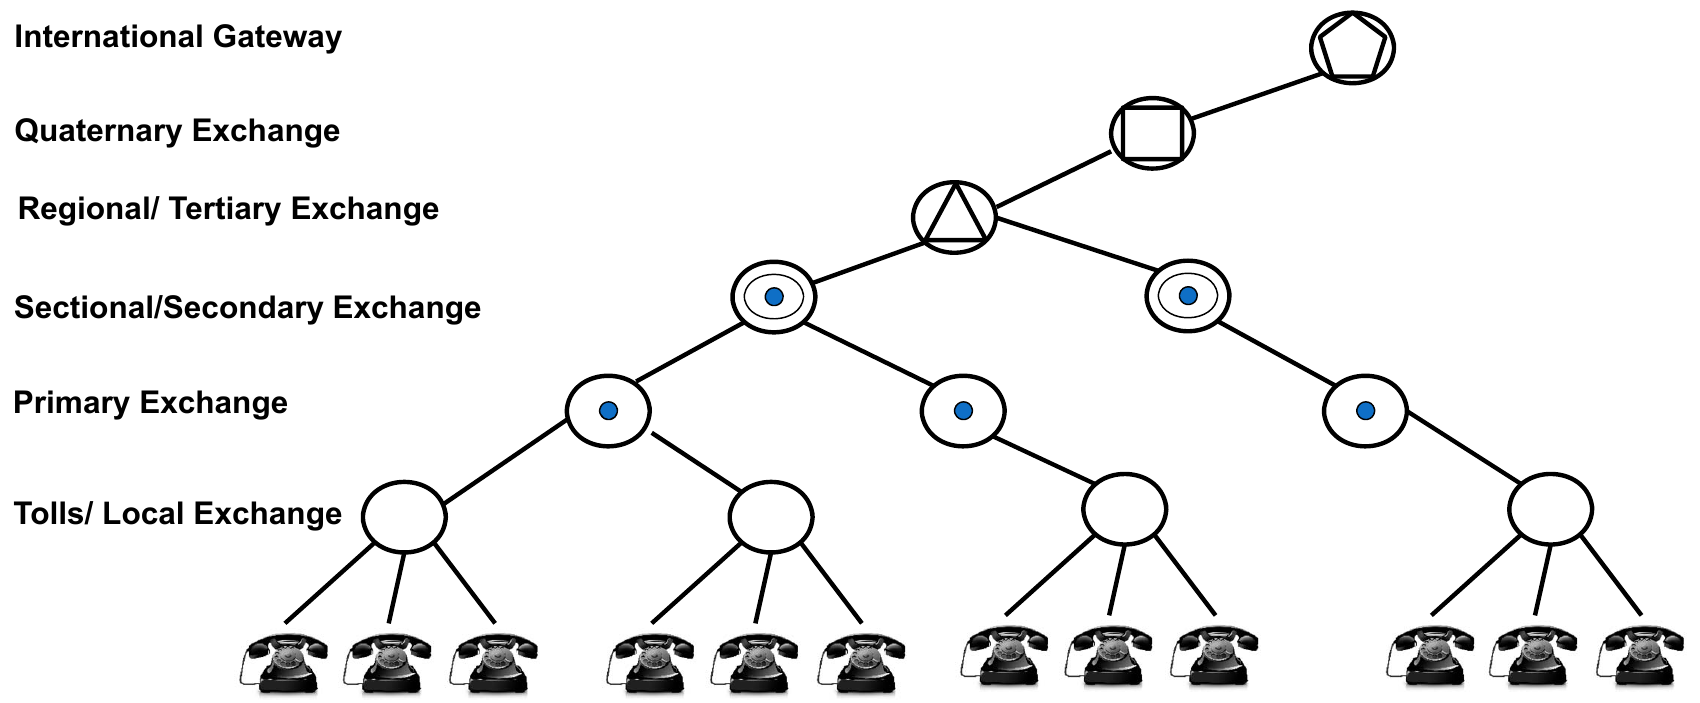
\includegraphics[
		width=14cm,
		%height=15cm
	]{images/Tema 2/Hierarchical network.png}
	\caption{
		\label{fig:unit2_hierarchy}
		Hierarchical network
	}
\end{figure}

The length of the end path depends on the distance between subscribers in the hierarchical network. For example, as shown in figure \ref{fig:unit2_dist_example}. Some paths would be:

\begin{itemize}
	\item $A \rightarrow B: A, CL1, B$
	\item $A \rightarrow C: A, CL1, CP1, CS2, CP2, CL2, C$
	\item $A \rightarrow D: A, CL1, CP1, CS2, CP2, CL3, D$
	\item $A \rightarrow E: A, CL1, CP1, CS2, CP2, CL3, E$
\end{itemize}

\begin{figure}[H]
	\centering
	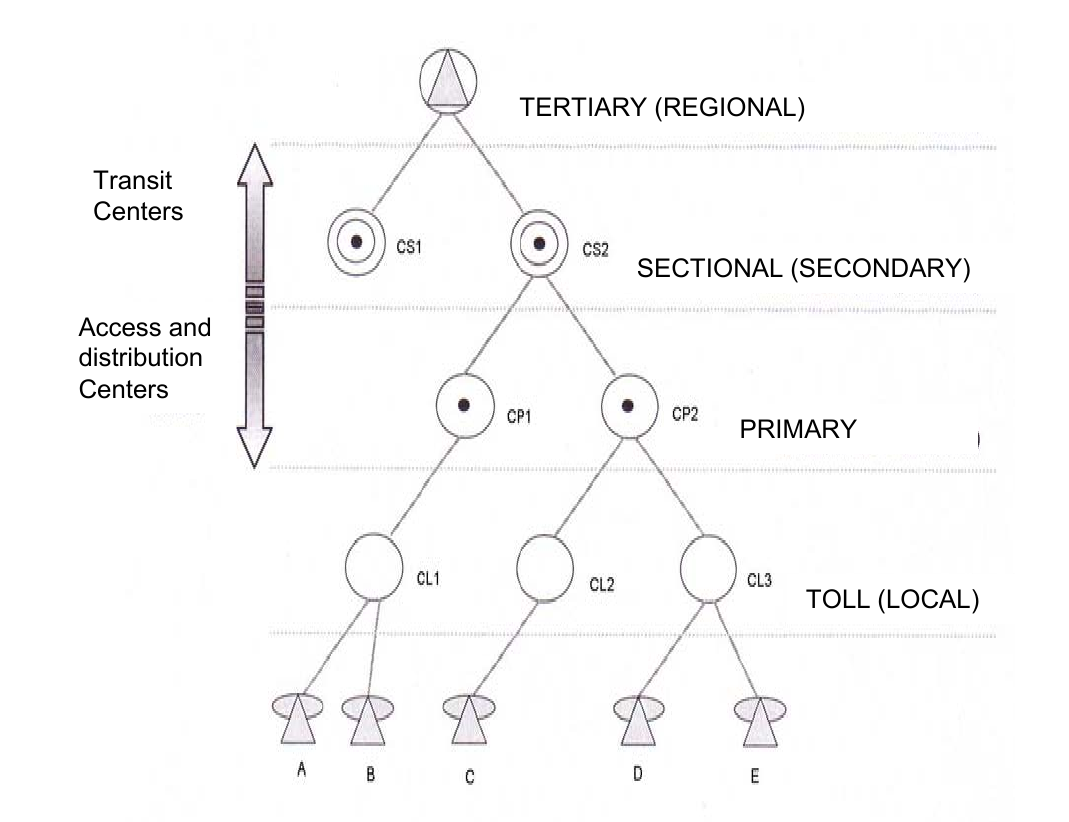
\includegraphics[
		width=12cm,
		%height=15cm
	]{images/Tema 2/Path distance example.png}
	\caption{
		\label{fig:unit2_dist_example}
		Path distance example
	}
\end{figure}

\subsubsection{High usage trunks}

The high usage trunks (HU) are superimposed to the hierarchical network. High usage trunks are
the direct sections and tandem centers. A direct section or high usage trunk is a set of links
interconnecting two exchanges that do not depend hierarchically. High usage trunks are selected
first for routing, and only when they are congested the traffic use final sections.

The following High Usage Trunks are allowed:

\begin{itemize}
	\item From toll to toll.
	\item From primary to primary.
	\item From sectional to sectional.
	\item From toll to primary that do not depend hierarchically.
	\item From primary to sectional that do not depend hierarchically.
	\item From sectional to regional that do not depend hierarchically.
\end{itemize}

\begin{figure}[H]
	\centering
	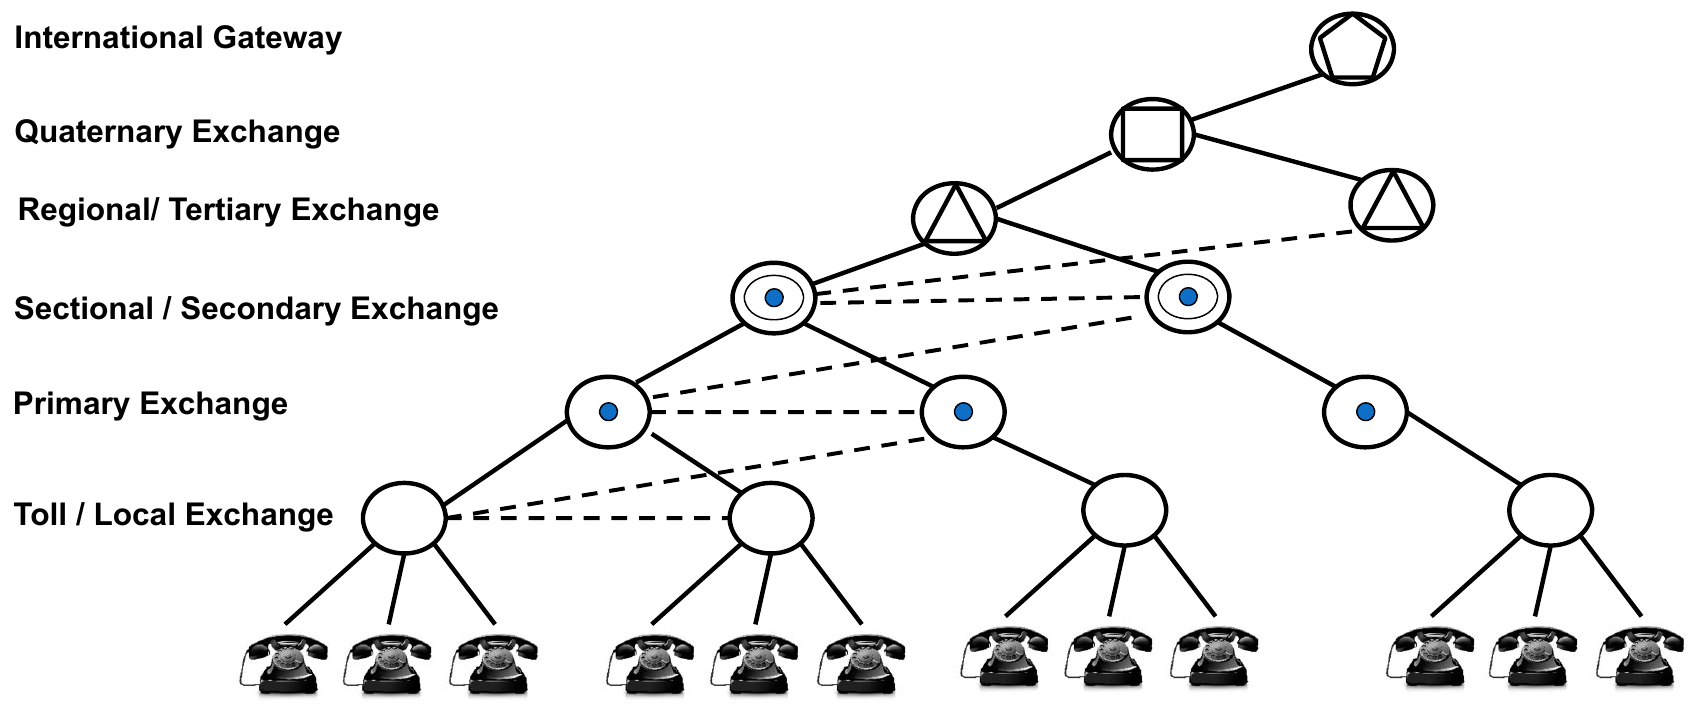
\includegraphics[
		width=14cm,
		%height=15cm
	]{images/Tema 2/High usage trunks.png}
	\caption{
		\label{fig:unit2_HU}
		High usage trunks
	}
\end{figure}

In very complex urban areas, there are tandem centers that are transit exchanges (without subscribers) connected to other exchanges. These tandem centers are not in the hierarchical network. Once the high usage trunks are present, the path between two subscribers is not unique.

\subsubsection{Routing}

The routing process through high ussage trunks can be decomposed in the following steps:

\begin{enumerate}
	\item Identify the destination tree.
	\item {
		In order to establish the route for the call, at each node I check if there is any high usage trunk (direct section) that brings me to a node in the destination tree and, if it is not congested, I select it. A series of criteria must be followed to select the correct HU:

		\begin{itemize}
			\item If there are several high usage trunks, take the one that brings me nearest.
			\item A route will not ever have two HUs, they can only be used once to reach the destination tree.
			\item {
				The route containing a HU can only have upward normal trunks before HU and downward normal trunks after HU, this is, the routes will always have the shape in figure \ref{fig:unit2_HU_route} or the opposite if it they are done from right to left.

				\begin{figure}[H]
					\centering
					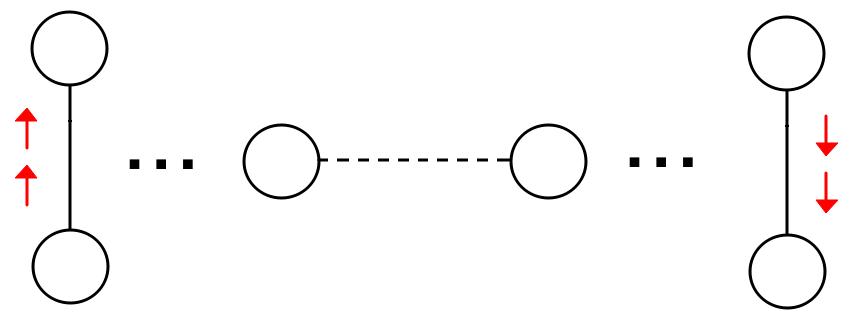
\includegraphics[
						width=7cm,
						%height=15cm
					]{images/Tema 2/HU.png}
					\caption{
						\label{fig:unit2_HU_route}
						Route containing a HU when going from left to right.
					}
				\end{figure}
			}
		\end{itemize}
	}
	\item If it is congested, I go up in hierarchy, since if any direct section (high usage trunk) has been selected, there is at least another path to the destination. One high usage trunk never overflows to another high usage trunk in the same node. This is, a high usage trunk always overflows to a final trunk. From that, we can establish a corollary: Only one high usage trunk is allowed per path.
	\item Once at the destination tree, we only can descend in hierarchy.
\end{enumerate}

For example, for the network shown in figure \ref{fig:unit2_routing_example}, routes would be:

\begin{itemize}
	\item $A \rightarrow C: AKC, AIKC, AINKC$
	\item $C \rightarrow A: CKA, CKNIA$
	\item $A \rightarrow F: AIPLF, AINLF, AINRPLF$
	\item $F \rightarrow A: FLNIA, FLPIA, FLPRNIA$
\end{itemize}

\begin{figure}[H]
	\centering
	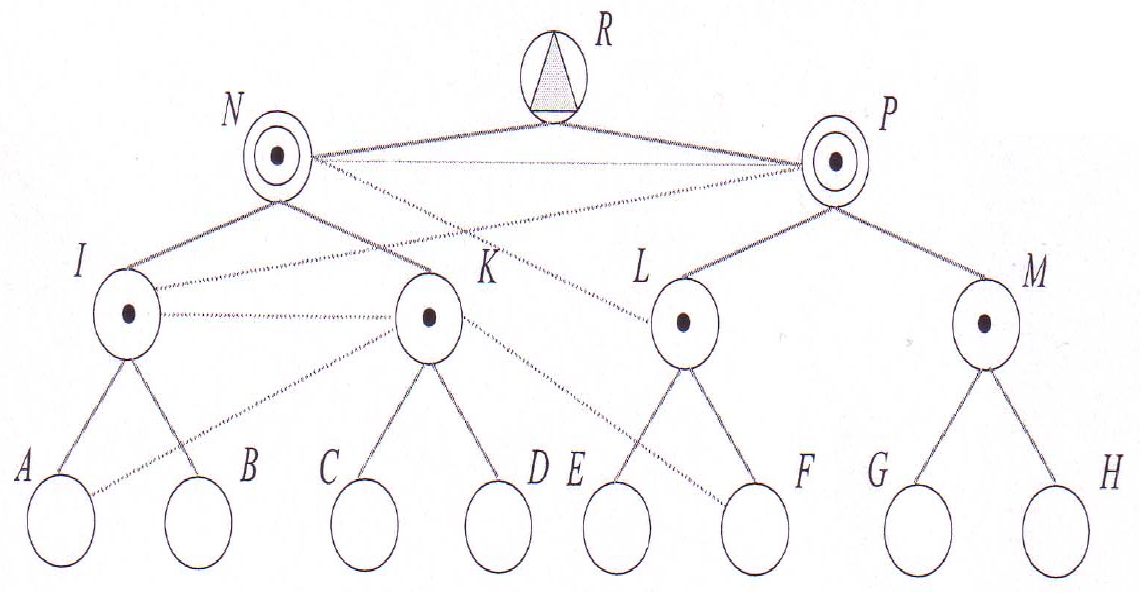
\includegraphics[
		width=10cm,
		%height=15cm
	]{images/Tema 2/Routing example.png}
	\caption{
		\label{fig:unit2_routing_example}
		Routing example
	}
\end{figure}

\subsubsection{Resultant traffic due to usage HU}

Due to the usage of HU, the resultant traffic both in HU and in FU is complex to estimate. The following scheme presents the different situations we will study:

\iffalse
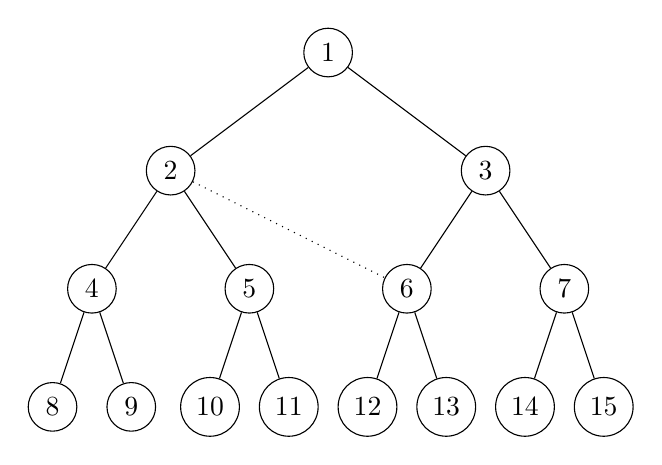
\begin{tikzpicture}[
  level distance=1.5cm,
  level 1/.style={sibling distance=4cm},
  level 2/.style={sibling distance=2cm},
  level 3/.style={sibling distance=1cm},
  level 4/.style={sibling distance=0.5cm},
  every node/.style={circle,draw}
  ]

% Root node
\node (n1) {1}
% Level 1
  child {node (n2) {2}
    % Level 2
    child {node (n4) {4}
      % Level 3
      child {node (n8) {8}}
      child {node (n9) {9}}
    }
    child {node (n5) {5}
      % Level 3
      child {node (n10) {10}}
      child {node (n11) {11}}
    }
  }
  child {node (n3) {3}
    % Level 2
    child {node (n6) {6}
      % Level 3
      child {node (n12) {12}}
      child {node (n13) {13}}
    }
    child {node (n7) {7}
      % Level 3
      child {node (n14) {14}}
      child {node (n15) {15}}
    }
  };

% Dotted line between nodes 2 and 6
\draw[dotted] (n2) -- (n6);

\end{tikzpicture}
\fi

\begin{figure}[H]
	\centering
	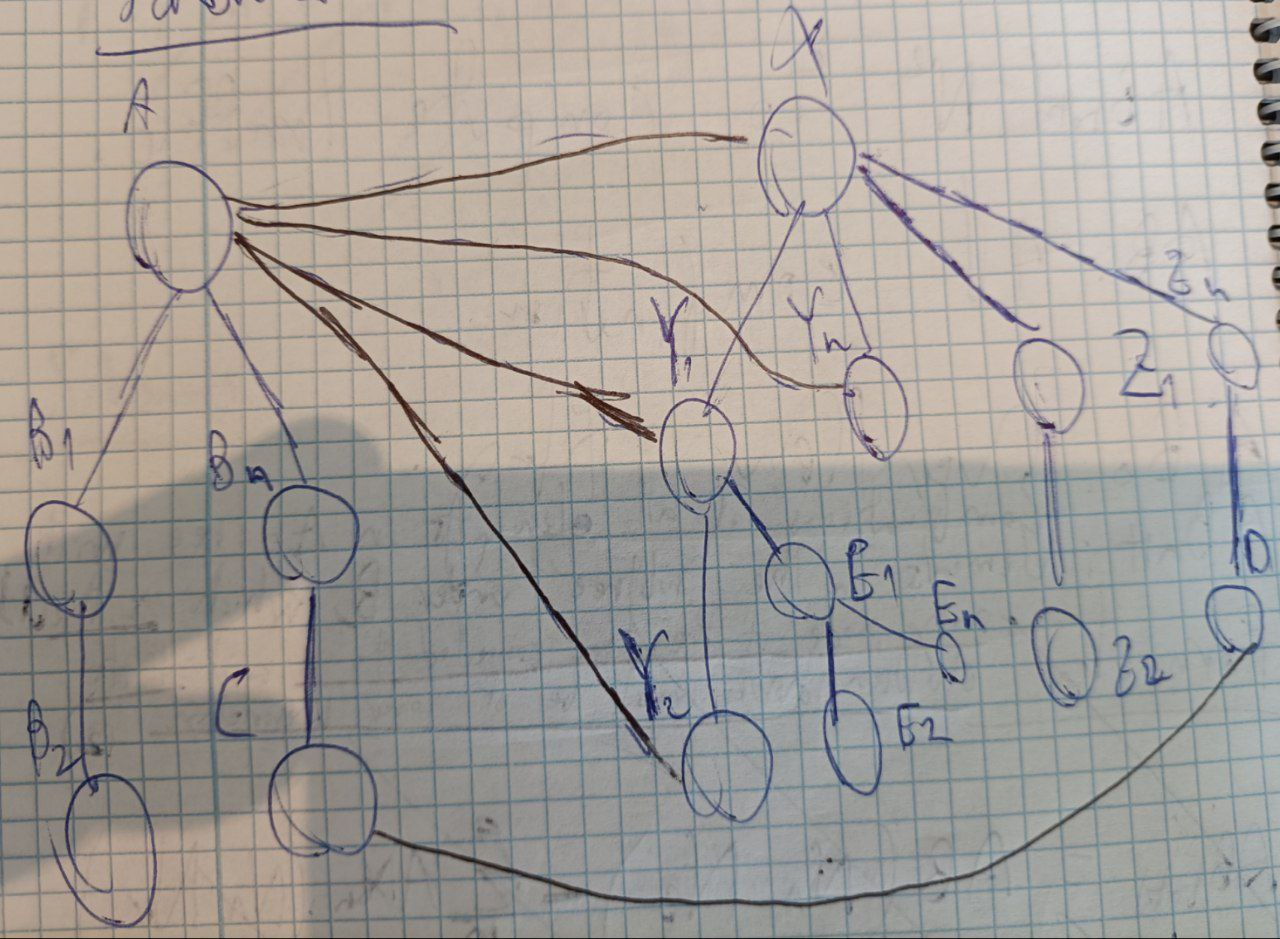
\includegraphics[
		width=12cm,
		%height=15cm
	]{images/Tema 2/network_scheme.jpg}
	\caption{
		\label{fig:unit2_network_scheme}
		Network scheme.
	}
\end{figure}

Here, in order to study HU between $A$ and $X$ we can distinguish:
\begin{itemize}
	\item Common HU ($AX$): Connects tree $A$ with tree $X$.
	\item Alternative HU ($AY$): Connects tree $A$ with tree $Y$ (a subtree from tree $X$), avoiding traffic going to $AX$.
	\item Lower hierarchy node with no alternative HU ($B$, $Z$): Always sends its traffic to $AX$/$XA$.
	\item Lower hierarchy node with alternative HU ($CD$): Traffic from $C$ to upper $D$ is send to $AX$ always; traffic from $C$ to lower $D$ is sent to $AX$ when saturation in HU.
\end{itemize}

\iffalse
Traffic calculation blablabla:

$$
	OT_{AX} = \sum_{AX} OT_{AX, own} + P_o \cdot \sum_{C, D} OT_{CD}
$$
\fi

In order to obtain the compute traffic at HU or FU we will use a recursive counting method to obtain all the components of the resultant traffic.

\paragraph{Traffic at HU}

The traffic at a HU can be computed in the following steps:
\begin{enumerate}
	\item Add the traffic from each node in tree $A$ to each node in tree $X$.
	\item Subtract the traffic that will be assisted by another HU ($alt$) connected to $A$.
	\item Subtract the traffic that will be assisted by another HU connected to a node from tree $A$, at a lower hierarchy.
	\item Add the traffic resulted by overflow ($o$) of previous HU connected to a node from tree $A$, at a lower hierarchy.
\end{enumerate}

The counting method to obtain the components for calculation will be:

$$
	AX_{total} = AX (N_A \cdot N_X) - \sum_Y AY_{alt} (N_A \cdot N_{YnoA}) + \sum_{C, D} \left( - CD_{alt} + CD_o (1) \right)
$$

Where:

\begin{itemize}
	\item $AX (N_A \cdot N_X) \rightarrow$ Traffic from each node in tree $A$ to each node in tree $X$.
	\item $\sum_Y AY_{alt} (N_A \cdot N_{YnoA}) \rightarrow$ Traffic that will be assisted by another HU connected to $A$.
	\item $\sum_{C, D} CD_{alt} \rightarrow$ Traffic that will be assisted by another HU connected to a node from tree $A$.
	\item $\sum_{C, D} CD_o (1) \rightarrow$ Traffic resulted by overflow of a HU connected to a node from tree $A$.
\end{itemize}

\iffalse
$$
	AX_{total} =
		\underset
			{\text{Traffic from each node in A to each node in B}}
			{\underbrace{AX (N_A \cdot N_X)}}
		\underset
			{\text{Iterations with alternative HUs}}
			{\underbrace{- \sum_Y AY_{alt} (N_A \cdot N_{YnoA})}}
		\underset
			{\text{Iterations with overflowing HUs}}
			{\underbrace{+ \sum_{C, D} \left( - CD_{alt} + CD_o (1) \right)}}
$$
\fi

\paragraph{Traffic at FU}

The traffic at a FU can be computed in the following steps:
\begin{enumerate}
	\item Add the traffic from each node in tree $A$ to each node in tree $X$.
	\item Subtract the traffic that will be assisted by another HU connected to a node from tree $A$.
	\item Add the traffic resulted by overflow ($o$) of previous HU connected to a node from tree $A$.
\end{enumerate}

The counting method to obtain the components for calculation will be:

$$
	AX_{total} = AX (N_A \cdot N_X) + \sum_{C, D} \left( - CD_{alt} + CD_o (1) \right)
$$

Where:

\begin{itemize}
	\item $AX (N_A \cdot N_X) \rightarrow$ Traffic from each node in tree $A$ to each node in tree $X$.
	\item $\sum_{C, D} CD_{alt} \rightarrow$ Traffic that will be assisted by another HU connected to a node from tree $A$.
	\item $\sum_{C, D} CD_o (1) \rightarrow$ Traffic resulted by overflow of a HU connected to a node from tree $A$.
\end{itemize}

\iffalse
$$
	AX_{total} =
		\underset
			{\text{Traffic from each node in A to each node in B}}
			{\underbrace{AX (N_A \cdot N_X)}}
		\underset
			{\text{Iterations with overflowing HUs}}
			{\underbrace{+ \sum_{C, D} \left( - CD_{alt} + CD_o (1) \right)}}
$$
\fi

\paragraph{Notation in counting methods}

\begin{itemize}
	\item $AB_{total}$: Number of elements to compute traffic in the HU that connects $A$ and $B$.
	\item $AB$: Size of the set with all the combinations of elements from $A$ tree and $B$ tree.
	\item $AB_o$: Element that indicates the traffic resulting from overflow in the HU that connects $A$ and $B$.
	\item {
		$AB_{alt}$: \textbf{Independent} combinations of elements in tree $A$ with elements in the limited subtree $B$ to compute the traffic in the HU between $A$ and $B$. We can consider two situations:
		\begin{itemize}
			\item {
				\textbf{$AB$ is an alternative to $AX$ and $B$ is in a lower hierarchy in tree $X$} $\rightarrow$ $AB_{alt}$ will represents the combinations of all elements in tree $A$ with elements in the limited subtree under $B$. The limited subtree under $B$ is defined by:
				\begin{itemize}
					\item $B$ is the only node of the tree connected to $A$.
					\item All its children nodes must be of lower hierarchy.
				\end{itemize}
			}
			\item {
				\textbf{$A$ is in the tree $X_1$ but in a lower hierarchy, $B$ is in the tree $X_2$ but in a higher hierarchy, so $AB$ overflows to $X_1 X_2$ partially} $\rightarrow$ $AB_{alt}$ will represents the independent combinations of all elements in tree $A$ with elements in the subtree under $B$ that exclusively overflow to $X_1 X_2$.
			}
		\end{itemize}
	}
\end{itemize}

The following relation can be useful:

\begin{itemize}
	\item $\sum_Y AY_{alt} (N_A \cdot N_{YnoA}) = AY_{highest} (N_A \cdot N_{Y_{highest}})$
	\item $N_{YnoA} = 1 + N_E$
\end{itemize}

\subsubsection{Concepts}

Two important concepts arise from the networks scenario:

\begin{itemize}
	\item {
		\textbf{Bid}

		Bid is the attempt to establish a conversation:

		\begin{itemize}
			\item Lifting a telephone.
			\item Partial dialing.
			\item Complete dialing, get the engage tone.
			\item Get ring tone back, no answer.
			\item Get ring tone back, answer.
		\end{itemize}

		Bids are the number of calls seized the circuits plus the number of calls rejected due to all circuits are busy assuming that there are no switching congestion.
	}
	\item {
		\textbf{Seizure}

		A seizure is a bid from d. It can be rejected or answered. Seizures are the number of calls answered plus the number of calls unanswered plus number of calls to busy plus subscribers plus the number of calls to recorded announcements.
	}
\end{itemize}

We can establish the following relation:

$$
	Bids > Seizures > Answers
$$

\subsection{Intelligent network}

The concept of intelligent network arised after the first efforts for digitalization of infrastructure. This would allow offering added value services such as:

\begin{itemize}
	\item Routing and number translations.
	\item Virtual Private Networks (VPNs).
	\item Special billing.
	\item Operator oriented services.
	\item etc.
\end{itemize}

The first standards were established in 1992 by ITU-T in the Q.1200 series recommendations.

Intelligent network is the basis for later telecommunication systems that use more complex networks, including access networks (ISDN, xDSL) and the backbone networks for mobile communications (GSM onwards).

\subsubsection{Architecture}

We must distinguish the following elements:

\begin{itemize}
	\item User equipment: Entry devices used by customers to request services to the network.
	\item Service Switching Point (SSP): It catches or switches incoming service requests. There is one per local exchange.
	\item Signalling Transfer Point (STP): It serves for interchange of signaling information among different parts of the telephony network.
	\item Service Control Point (SCP): It consists in a stand alone computer connected to a database. It checks up the services and made corresponding requests.
	\item External Data Base (DB): The SCP might need to use an external data base for certain services. For example, a credit card data base.
	\item Adjunct: Same functions as SCP but is contained in a local exchange. In this way, intelligent functions are partially decentralized and higher level instances manage less load.
	\item {
		Intelligent Peripheral (IP): It has several functions related to incoming service requests:
		\begin{itemize}
			\item Voice synthesis, either from already stored text messages or text to voice conversion.
			\item Voice recognition that allows users to answer questions or select options (numbers, yes or no, ...).
			\item Voice recording such as voice mailbox.
			\item Multi-frequency digit recognition at second dialing phase.
		\end{itemize}
	}
	\item Service Management System (SMS): From this point of the network, services are controlled, providing technical and commercial management for intelligent network. This is done by giving complete and secure information to each SCP (sink for statistical data, service measurements, alarms, ...). It does not need real time connections.
	\item {
		Service Creation Environment Point (SCE/P): From this point of the network, new services are implemented. This is done through several stages:
		\begin{itemize}
			\item {
				Formal service specification:
				\begin{itemize}
					\item Service development.
					\item Service verification.
					\item Service simulation.
				\end{itemize}
			}
			\item Service implantation.
		\end{itemize}
		 It does not need real time connections.
	}
\end{itemize}

\begin{figure}[H]
	\centering
	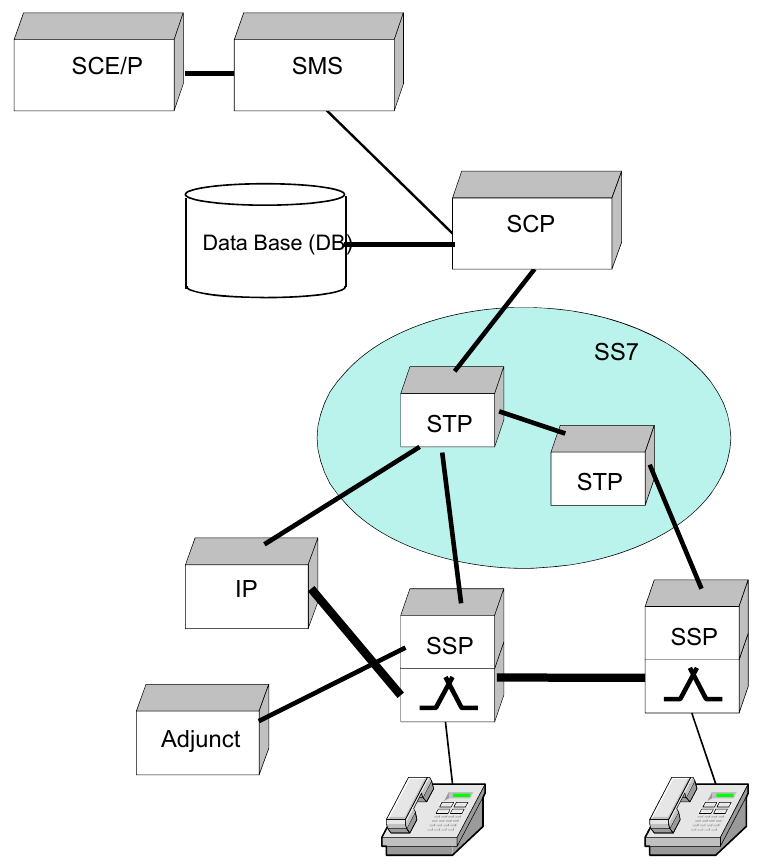
\includegraphics[
		width=12cm,
		%height=15cm
	]{images/Tema 2/Intelligent network.png}
	\caption{
		\label{fig:unit2_int_net}
		Intelligent network scheme
	}
\end{figure}

\section{Multiplexing and multiple access}

\subsection{Introduction}

As studied, multiplexing and multiple access are two fundamental strategies to manage the network usage, which is limited. The way in which these strategies strategies are implemented results in different performances which can be modeled.

\subsection{Network parameters}

The study of multiplexing and multiple access requires the following parameters:

\begin{itemize}
	\item Incoming traffic ($I$): It is the traffic offered to users.
	\item Retransmissions ($R$): It is the traffic resulted from retransmissions, packets that failed to be transmitted in the first try.
	\item {
		Traffic inputed to the network ($G$):

		$G = I + R$
	}
	\item {
		Network efficiency ($S$): Traffic that is outputed. It can be computed from offered traffic to the net in relation with offered traffic from users and retransmissions:

		$S = S(G, I , R)$

		If there is no congestion, it equals offered traffic:

		$S \overset{\text{(no congestion)}}{=} I \rightarrow G = S + R$
	}
\end{itemize}

\begin{figure}[H]
	\centering
	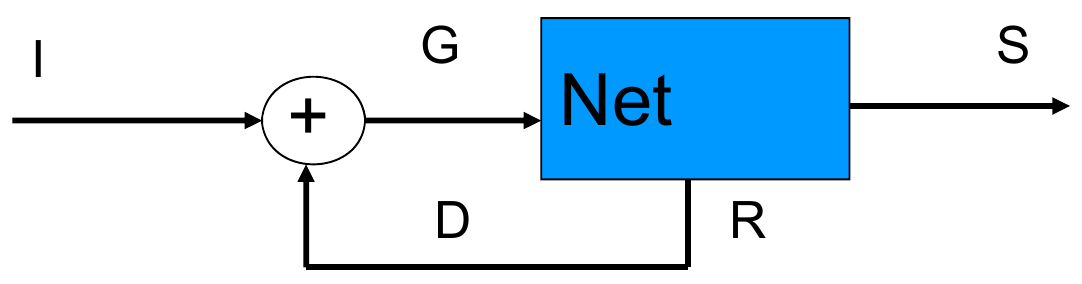
\includegraphics[
		width=10cm,
		%height=15cm
	]{images/Tema 2/Multiplexing and multiple access.png}
	\caption{
		\label{fig:unit2_mul}
		Scheme of network traffic
	}
\end{figure}

Previous measures can be normalized to network efficiency $S$, so instead of Erlangs, they will be packets (transmissions) per packet:

$$
	\overline{I} = \frac {I} {S} \overset{\text{(no congestion)}}{=} 1
$$

$$
	\overline{R} = \frac {R} {S}
$$

$$
	\overline{G} = \frac {G} {S} = \overline{I} + \overline{R} = \frac {I + R} {S}
$$

In this way, $\frac {S}{G}$ indicates the probability of successfully transmitting a packet and $\frac {G}{S}$ is the average needed retransmissions to successfully transmit a packet.

\subsection{Packet transmission}

Network scenarios will also be characterized by packet transmission properties:

\begin{itemize}
	\item {
		Packet propagation ($t_p$): It is the normalized propagation time.

		$a = \frac {t_p} {W_s}$
	}
	\item {
		Generating acknowledgement ($t_{ACK}$): It is the normalized acknowledgement time.

		$w = \frac {t_{ACK}} {W_s}$
	}
	\item {
		Transmission delay ($D$): It is the normalized delay.

		$D = \frac {t_{tx}} {W_s}$
	}
\end{itemize}

\subsection{Access protocols}

To solve multiplexing and multiple access problem, several access protocols have been developed.

\subsubsection{Centralized Aloha}

It was invented at the Hawaii University in 1970. There is a distributed variant, but since packet propagation ($a$) is usually small, the centralized version is commonly used for both scenarios.

Its operation can be summarized in:

\begin{itemize}
	\item If the terminal wants to transmit, it does and waits for the acknowledgement.
	\item If the acknowledgement is not received, it retransmits waiting a random time between $1$ and $k$.
\end{itemize}

\begin{figure}[H]
	\centering
	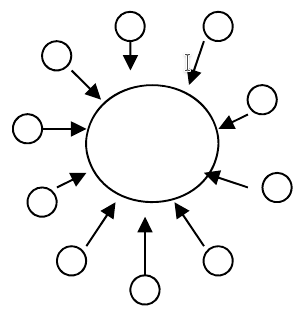
\includegraphics[
		width=5cm,
		%height=15cm
	]{images/Tema 2/Centralized.png}
	\caption{
		\label{fig:unit2_cen_aloha_sheme}
		Centralized Aloha scheme
	}
\end{figure}

Its characteristics are:

\begin{itemize}
	\item {
		Transmission delay:

		$
			D =
			\left( \frac {G} {S} - 1 \right) \cdot \left( \frac {k+1} {2} + 1 + 2a + w \right) + a + 1 \overset{\frac {G} {S} = e^{2G}}{=}
			\left( e^{2G} - 1 \right) \cdot \left( \frac {k+1} {2} + 1 + 2a + w \right) + a + 1
		$
	}
	\item {
		Network efficiency: Assuming Poisson arrivals, we have:

		$
			S = G \cdot e^{-2G}
		$

		Its maximum value, for $G = 0.5$ is:

		$
			S_{MAX} = 0.5 e^{-1} = 0.184
		$
	}
\end{itemize}

\begin{figure}[H]
	\centering
	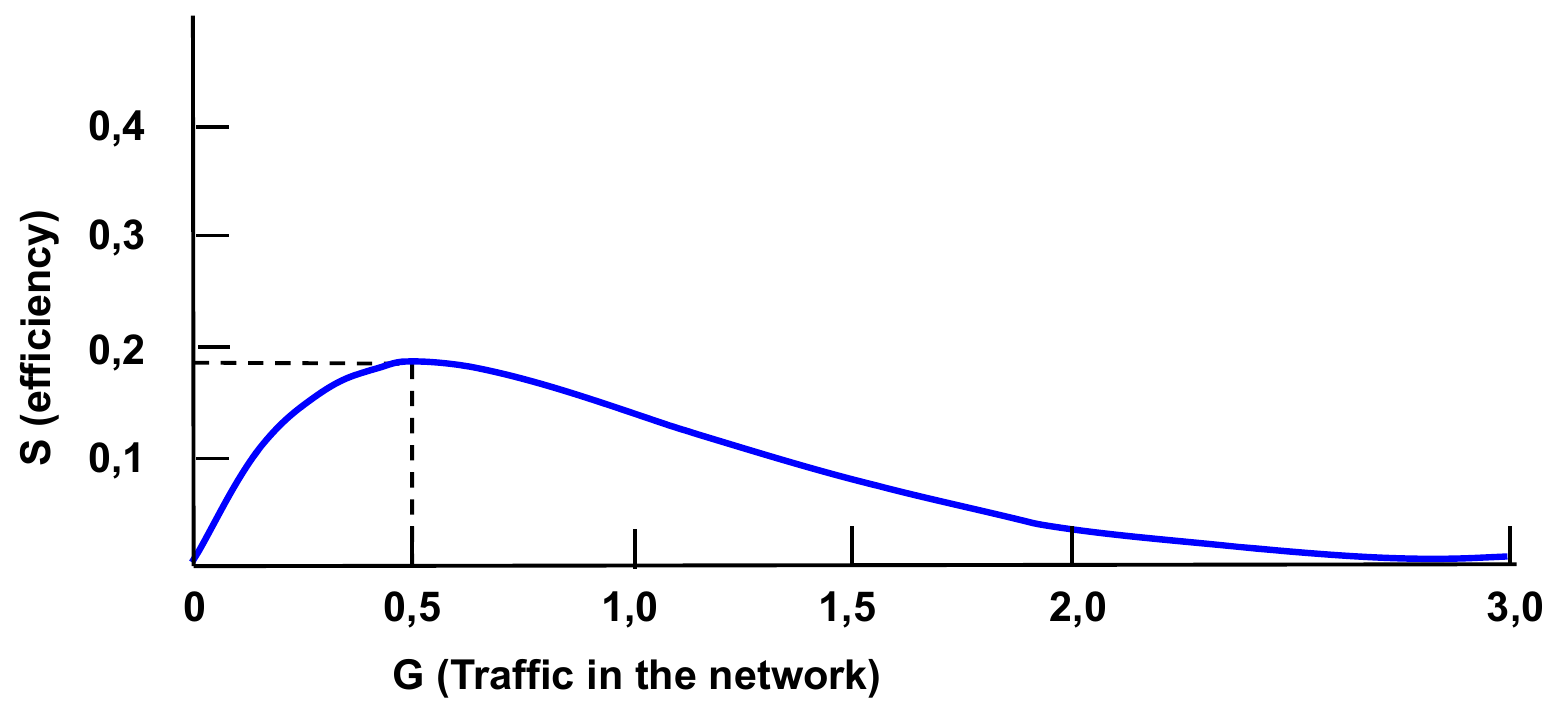
\includegraphics[
		width=12cm,
		%height=15cm
	]{images/Tema 2/Centralized Aloha S.png}
	\caption{
		\label{fig:unit2_cen_aloha_S}
		Centralized Aloha efficiency
	}
\end{figure}

\subsubsection{Distributed Aloha}

\begin{figure}[H]
	\centering
	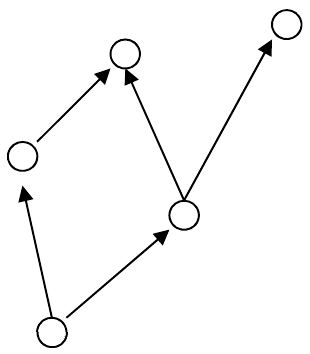
\includegraphics[
		width=5cm,
		%height=15cm
	]{images/Tema 2/Distributed.png}
	\caption{
		\label{fig:unit2_dis_aloha_sheme}
		Distributed Aloha scheme
	}
\end{figure}

It is distributed. Its characteristics are:

\begin{itemize}
	\item {
		Transmission delay:

		$
			D =
			\left( \frac {G} {S} - 1 \right) \cdot \left( \frac {k+1} {2} + 1 + 2a + w \right) + a + 1 \overset{\frac {G} {S} = e^{2G \cdot (1+a)}}{=}
			\left( e^{2G \cdot (1+a)} - 1 \right) \cdot \left( \frac {k+1} {2} + 1 + 2a + w \right) + a + 1
		$
	}
	\item {
		Network efficiency: Assuming Poisson arrivals, we have:

		$
			S = G \cdot e^{-2G \cdot (1+a)}
		$
		Its maximum value, for $G = \frac {1} {2 (1+a)}$ is:

		$
			S_{MAX} = \frac {1} {2 (1+a) e}
		$
	}
\end{itemize}

\subsubsection{Slotted Aloha}

It is an improvement on simple Aloha to solve collisions problem. Its operation can be summarized in:

\begin{itemize}
	\item The time is divided into slots.
	\item Only transmission at the beginning of the slots is allowed.
\end{itemize}

\begin{figure}[H]
	\centering
	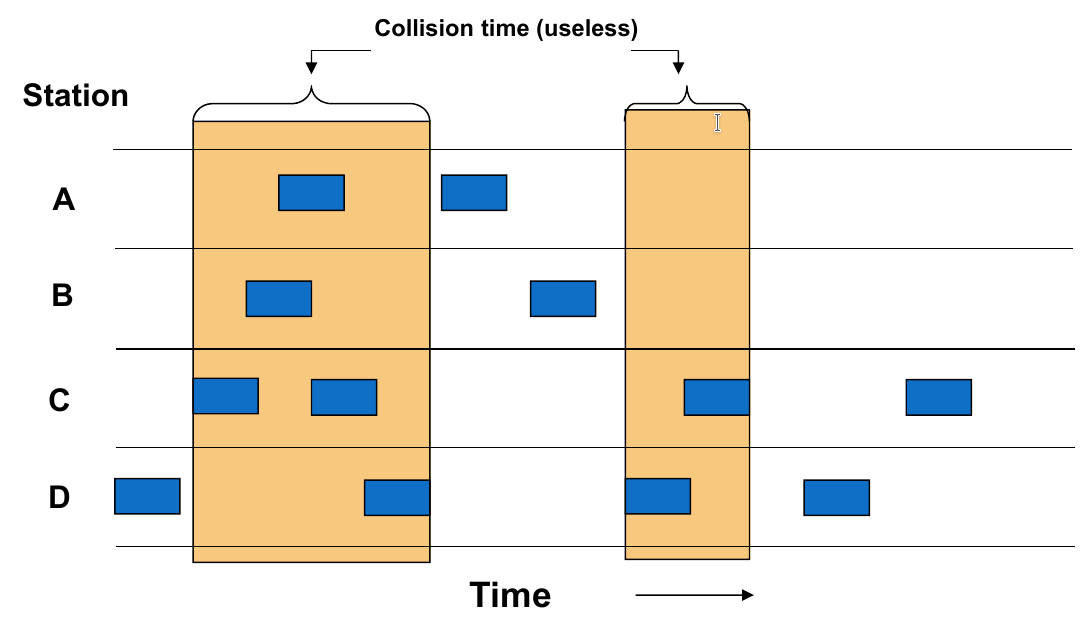
\includegraphics[
		width=14cm,
		%height=15cm
	]{images/Tema 2/Slotted Aloha.png}
	\caption{
		\label{fig:unit2_slo_aloha_sheme}
		Slotted Aloha scheme
	}
\end{figure}

Its characteristics are:

\begin{itemize}
	\item {
		Packet propagation: It is the normalized propagation time ($t_p$). So:

		$
			a = \frac {t_p} {W_s}
		$
	}
	\item {
		Generating acknowledgement: It is the normalized acknowledgement time ($t_{ACK}$). So:

		$
			w = \frac {t_{ACK}} {W_s}
		$
	}
	\item {
		Transmission delay:

		$
			D =
			\left( \frac {G} {S} - 1 \right) \cdot \left( \frac {k+1} {2} + 1.5 + 2a + w \right) + a + 1.5 \overset{\frac {G} {S} = e^G}{=}
			\left( e^G - 1 \right) \cdot \left( \frac {k+1} {2} + 1.5 + 2a + w \right) + a + 1.5
		$
	}
	\item {
		Offered traffic to the net:

		$
			G = S + R
		$
	}
	\item {
		Network efficiency: Assuming Poisson arrivals, we have:

		$
			S = G \cdot e^{-G}
		$

		Its maximum value, for $G = 1$, is:

		$
			S_{MAX} = e^{-1} = 0.368
		$
	}
\end{itemize}

\begin{figure}[H]
	\centering
	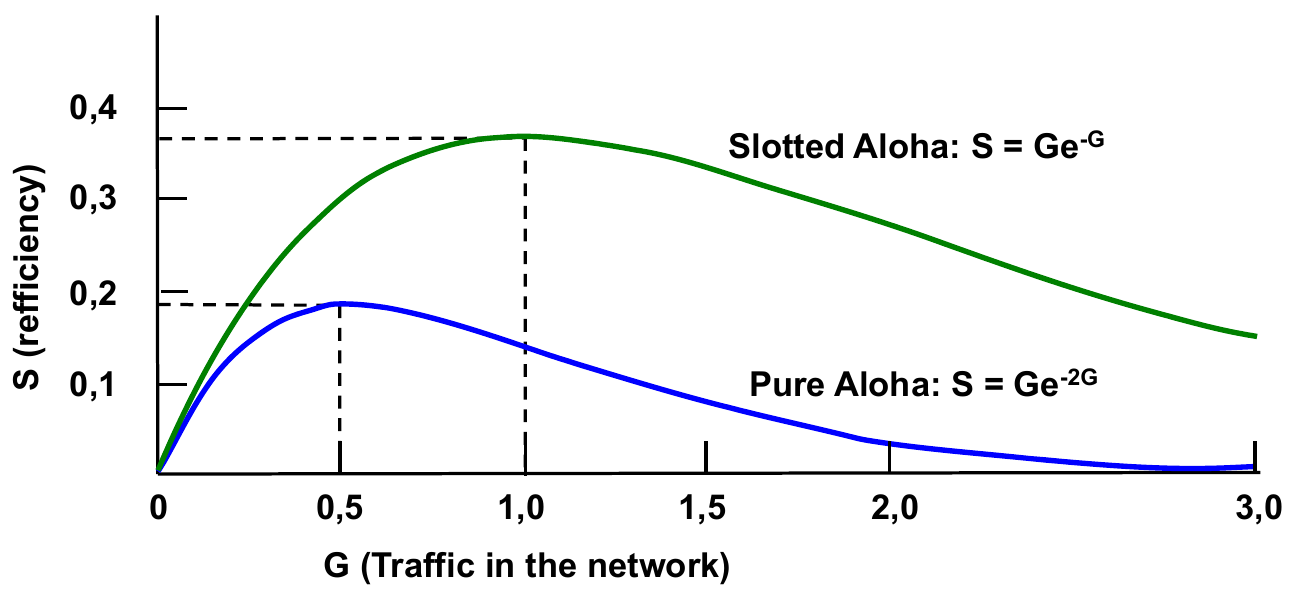
\includegraphics[
		width=12cm,
		%height=15cm
	]{images/Tema 2/Aloha comparison.png}
	\caption{
		\label{fig:unit2_aloha_comp}
		Aloha comparison
	}
\end{figure}

\subsubsection{Carrier Sense Multiple Access (CSMA)}

Before transmission, the channel is sensed:

\begin{itemize}
	\item Before transmitting, channel is listen.
	\item If no one is transmitting, it transmits.
	\item {
		If the channel is busy:
		\begin{itemize}
			\item {
				Non-persistent: It waits a random time and then, the process starts.

				$
					S = \frac {G} {G+1}
				$
			}
			\item {
				1-persistent: It waits until the channel is free and it transmits once it is. If collision, again 1-persistent.

				$
					S = \frac {G \cdot (1 + G) \cdot e^{-G}} {G + e^{-G}}
				$

				$
					S_{MAX} = 0.55
				$
			}
			\item $p$-persistent: It waits with probability $1 - p$ and transmits with probability $p$.
		\end{itemize}
	}
\end{itemize}

\begin{figure}[H]
	\centering
	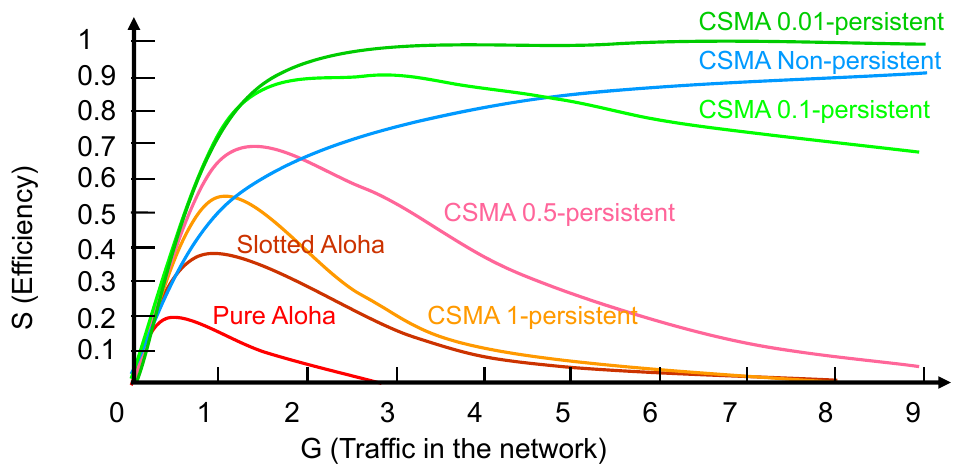
\includegraphics[
		width=12cm,
		%height=15cm
	]{images/Tema 2/All comparison.png}
	\caption{
		\label{fig:unit2_all_comp}
		Comparison of all transmission protocols
	}
\end{figure}

\subsection{Summary}

\subsubsection{Network parameters}

$G = I + R$, 
$S \overset{\text{(no congestion)}}{=} I \rightarrow G = S + R$

$\overline{I} = \frac {I} {S} \overset{\text{(no congestion)}}{=} 1$, 
$\overline{R} = \frac {R} {S}$, 
$\overline{G} = \frac {G} {S} = \overline{I} + \overline{R} = \frac {I + R} {S}$

\subsubsection{Packet transmission}

$a = \frac {t_p} {W_s}$, 
$w = \frac {t_{ACK}} {W_s}$, 
$D = \frac {t_{tx}} {W_s}$

\subsubsection{Access protocols}

\begin{tabular}{|p{2cm}|c|c|p{8cm}|}
	\hline
	& $S$ & $S_{MAX}$ & $D$ \\
	\hline
	Aloha & $G \cdot e^{-2G}$ & $0.5 e^{-1} = 0.184$ & $\left( \frac {G} {S} - 1 \right) \cdot \left( \frac {k+1} {2} + 1 + 2a + w \right) + a + 1 \overset{\frac {G} {S} = e^{2G}}{=} \left( e^{2G} - 1 \right) \cdot \left( \frac {k+1} {2} + 1 + 2a + w \right) + a + 1$ \\
	\hline
	Distributed Aloha & $G \cdot e^{-2G \cdot (1+a)}$ & $\frac {1} {2 (1+a) e}$ & $\left( \frac {G} {S} - 1 \right) \cdot \left( \frac {k+1} {2} + 1 + 2a + w \right) + a + 1 \overset{\frac {G} {S} = e^{2G \cdot (1+a)}}{=} \left( e^{2G \cdot (1+a)} - 1 \right) \cdot \left( \frac {k+1} {2} + 1 + 2a + w \right) + a + 1$ \\
	\hline
	Slotted Aloha & $G \cdot e^{-G}$ & $e^{-1} = 0.368$ & $\left( \frac {G} {S} - 1 \right) \cdot \left( \frac {k+1} {2} + 1.5 + 2a + w \right) + a + 1.5 \overset{\frac {G} {S} = e^G}{=} \left( e^G - 1 \right) \cdot \left( \frac {k+1} {2} + 1.5 + 2a + w \right) + a + 1.5$ \\
	\hline
	CSMA (Non-persistent) & $\frac {G} {G+1}$ & & \\
	\hline
	CSMA (1-persistent) & $\frac {G \cdot (1 + G) \cdot e^{-G}} {G + e^{-G}}$ & $0.55$ & \\
	\hline
	CSMA ($p$-persistent) & & & \\
	\hline
\end{tabular}

\begin{landscape}

\begin{tabular}{|c|p{8cm}|}
	\hline
	& $D$ \\
	\hline
	Aloha & $\left( \frac {G} {S} - 1 \right) \cdot \left( \frac {k+1} {2} + 1 + 2a + w \right) + a + 1 \overset{\frac {G} {S} = e^{2G}}{=} \left( e^{2G} - 1 \right) \cdot \left( \frac {k+1} {2} + 1 + 2a + w \right) + a + 1$ \\
	\hline
	Distributed Aloha & $\left( \frac {G} {S} - 1 \right) \cdot \left( \frac {k+1} {2} + 1 + 2a + w \right) + a + 1 \overset{\frac {G} {S} = e^{2G \cdot (1+a)}}{=} \left( e^{2G \cdot (1+a)} - 1 \right) \cdot \left( \frac {k+1} {2} + 1 + 2a + w \right) + a + 1$ \\
	\hline
	Slotted Aloha & $\left( \frac {G} {S} - 1 \right) \cdot \left( \frac {k+1} {2} + 1.5 + 2a + w \right) + a + 1.5 \overset{\frac {G} {S} = e^G}{=} \left( e^G - 1 \right) \cdot \left( \frac {k+1} {2} + 1.5 + 2a + w \right) + a + 1.5$ \\
	\hline
	CSMA (Non-persistent) & \\
	\hline
	CSMA (1-persistent) & \\
	\hline
	CSMA ($p$-persistent) & \\
	\hline
\end{tabular}

\end{landscape}

\section{Link budget and transmission}

\subsection{Power and decibels}

\subsubsection{Definition}

Decibels are always obtained from a relation:

$$
	c = \frac {a} {b} \rightarrow c_{dB} = 10 \log (c) = 10 \log \left( \frac {a} {b} \right) = 10 \log (a) - 10 \log (b) = a_{dB} - b_{dB}
$$

They are commonly used to represent concepts related to power since they usually imply two quatities we can relate. For example, gains and losses (power of a signal before and after transmission).

\subsubsection{Reference and conversion}

Absolute values need a reference:

\begin{itemize}
	\item $dBW$: Referred to Watts ($W$)
	\item $dBm$: Referred to $mW$
	\item $dB\mu$: Referred to $\mu W$
\end{itemize}

Since the relation between them is an order of 3 ($30 dB$), we can convert between them by adding and subtracting $30 dB$.

\begin{figure}[H]
	\centering
	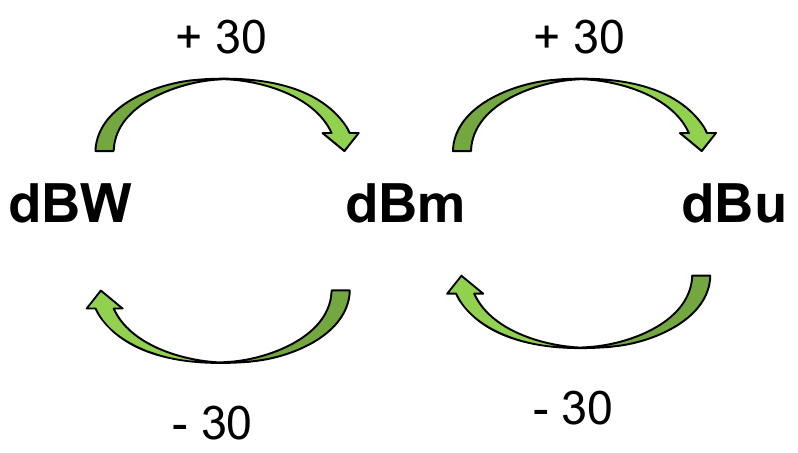
\includegraphics[
		width=6cm,
		%height=15cm
	]{images/Tema 2/Decibels conversion.png}
	\caption{
		\label{fig:unit2_dedibels}
		Decibels conversion
	}
\end{figure}

\subsection{Gains and losses}

When a signal is transmitted ($p_{tx}$), it can be amplified with a certain gain ($g$) or suffer losses ($l$). The resulting power ($p_{rx}$) is the product by gains and division by losses:

$$
	p_{rx} = p_{tx} \cdot \frac {\prod_i g_i} {\prod_i l_i}
$$

It is usually expressed in decibels:

$$
	P_{rx} = T_{tx} + \sum_i G_i - \sum_j L_j
$$

Where:

\begin{itemize}
	\item $P_{tx} = 10 \log (p_{tx})$
	\item $P_{rx} = 10 \log (p_{rx})$
	\item $G_i = 10 \log (g_i)$
	\item $L_i = 10 \log (l_i)$
\end{itemize}

\subsection{Propagation}

\subsubsection{Total propagation losses (in decibels)}

$$
	l_b = l_{bf} \cdot a_E
$$

$$
	L_b = L_{bf} + A_E
$$

Where:

\begin{itemize}
	\item Free-space path loss: $l_{bf}$
	\item Losses due to other factors: $a_E$
\end{itemize}

\subsubsection{Free-space path loss}

$$
	l_{bf} = \left( \frac {4 \pi d} {\lambda} \right)^2
$$

$$
	L_{bf} = 10 \log \left[ \left( \frac {4 \pi d} {\lambda} \right)^2 \right]
$$

Where:

\begin{itemize}
	\item Distance to antenna: $d$
	\item Wavelength: $\lambda$
\end{itemize}

\subsubsection{Free-space path loss (variable index)}

$$
	l_{bf} = \left( \frac {4 \pi d} {\lambda} \right)^n
$$

$$
	L_{bf} = 10 \log \left[ \left( \frac {4 \pi d} {\lambda} \right)^n \right]
$$

Where:

\begin{itemize}
	\item Distance to antenna: $d$
	\item Wavelength: $\lambda$
	\item Propagation index: $n$
\end{itemize}

\subsubsection{Antenna gain}

$$
	g = \eta \left( \frac {\pi D} {\lambda} \right)^2
$$

$$
	G = 10 \log \left[ \eta \left( \frac {\pi D} {\lambda} \right)^2 \right]
$$

Where:

\begin{itemize}
	\item Antenna diameter: $D$
	\item Wavelength: $\lambda$
	\item Antenna efficiency: $\eta$
\end{itemize}

\subsection{Interference}

\subsubsection{Noise power spectral density (adjusted to bandwidth)}

$$
	p_N = N = N_0 B = k T_0 B
$$

$$
	P_N = N_{dB} = 10 \log (N_0) + 10 \log (B) = 10 \log (k T_0 B)
$$

Where:

\begin{itemize}
	\item Boltzman constant: $k = 1.38 \cdot 10^{-23} [J/K]$
	\item Receiver system noise temperature in kelvins: $T_0$
	\item Channel bandwidth: $B$
\end{itemize}

\subsubsection{Carrier-to-noise ratio}

$$
	\left( \frac {C} {N} \right) = \frac {p_{rx}} {k T_0 B}
$$

$$
	\left( \frac {C} {N} \right)_{dB} = P_{rx} + 10 \log \left( \frac {1} {T_0} \right) - 10 \log (k B)
$$

Where:

\begin{itemize}
	\item Boltzman constant: $k = 1.38 \cdot 10^{-23} [J/K]$
	\item Receiver system noise temperature in kelvins: $T_0$
	\item Noise power spectral density: $N_0$
	\item Noise power spectral density (adjusted to bandwidth): $N$
	\item Carrier signal average power: $C$
	\item Channel bandwidth: $B$
	\item Data rate: $R_b$
\end{itemize}

\subsubsection{Energy per bit to noise ratio}

$$
	\frac {E_b} {N_0} = \frac {C} {N} \frac {B} {R_b} = \frac {C} {N_0} \frac {1} {R_b}
$$

Where:

\begin{itemize}
	\item Energy per bit: $E_b$
	\item Noise power spectral density: $N_0$
	\item Noise power spectral density (adjusted to bandwidth): $N$
	\item Carrier signal average power: $C$
	\item Channel bandwidth: $B$
	\item Data rate: $R_b$
\end{itemize}



\end{document}
